%!TEX root = ../template.tex
%%%%%%%%%%%%%%%%%%%%%%%%%%%%%%%%%%%%%%%%%%%%%%%%%%%%%%%%%%%%%%%%%%%%
%% chapter4.tex
%% NOVA thesis document file
%%
%% Chapter with the system architecture
%%%%%%%%%%%%%%%%%%%%%%%%%%%%%%%%%%%%%%%%%%%%%%%%%%%%%%%%%%%%%%%%%%%%
\chapter{System Architecture}
\label{cha:system_architecture}

\begin{quotation}
\begin{flushright}
\itshape
«missing quote...»\\
\textbf{- Author}
\end{flushright}
\end{quotation}

On this chapter, the complete system architecture will be presented, starting by describing the system requirements based on the thesis goal. It will followed by an introduction to the main system components, and end with a detailed description of the system's architecture layers.

% ==========================
% = System requirements =
% ==========================

\section{System Requirements}
\label{sec:system_architecture_requirements}

In order to properly develop the present work, the system's requirements must be considered. The first question that needs to be asked is

\begin{quotation}
\textbf{Considering the goal of doing 3D bioprinting in situ into burn wounds, what are the requirements for developing this system?}
\end{quotation}

In general terms, this system must have into consideration requirements associated with the particular needs of bioprinting like resolution, and bioprinting method. It should also consider the particularities of how to position the print head within the wound area. Depending on the degree of autonomy, we should also consider how the wounds will be detected and referenced within the positioning system. Physical constraints like dimensions and weight are also important. Lastly, but also vital are the safety requirements. A more complete list of the main requirements for this system, by category, is presented:

{\color{red}Mention the paper that talks about the future requirements of 3D bioprinting.}

\begin{figure}[htbp]
	\centering
	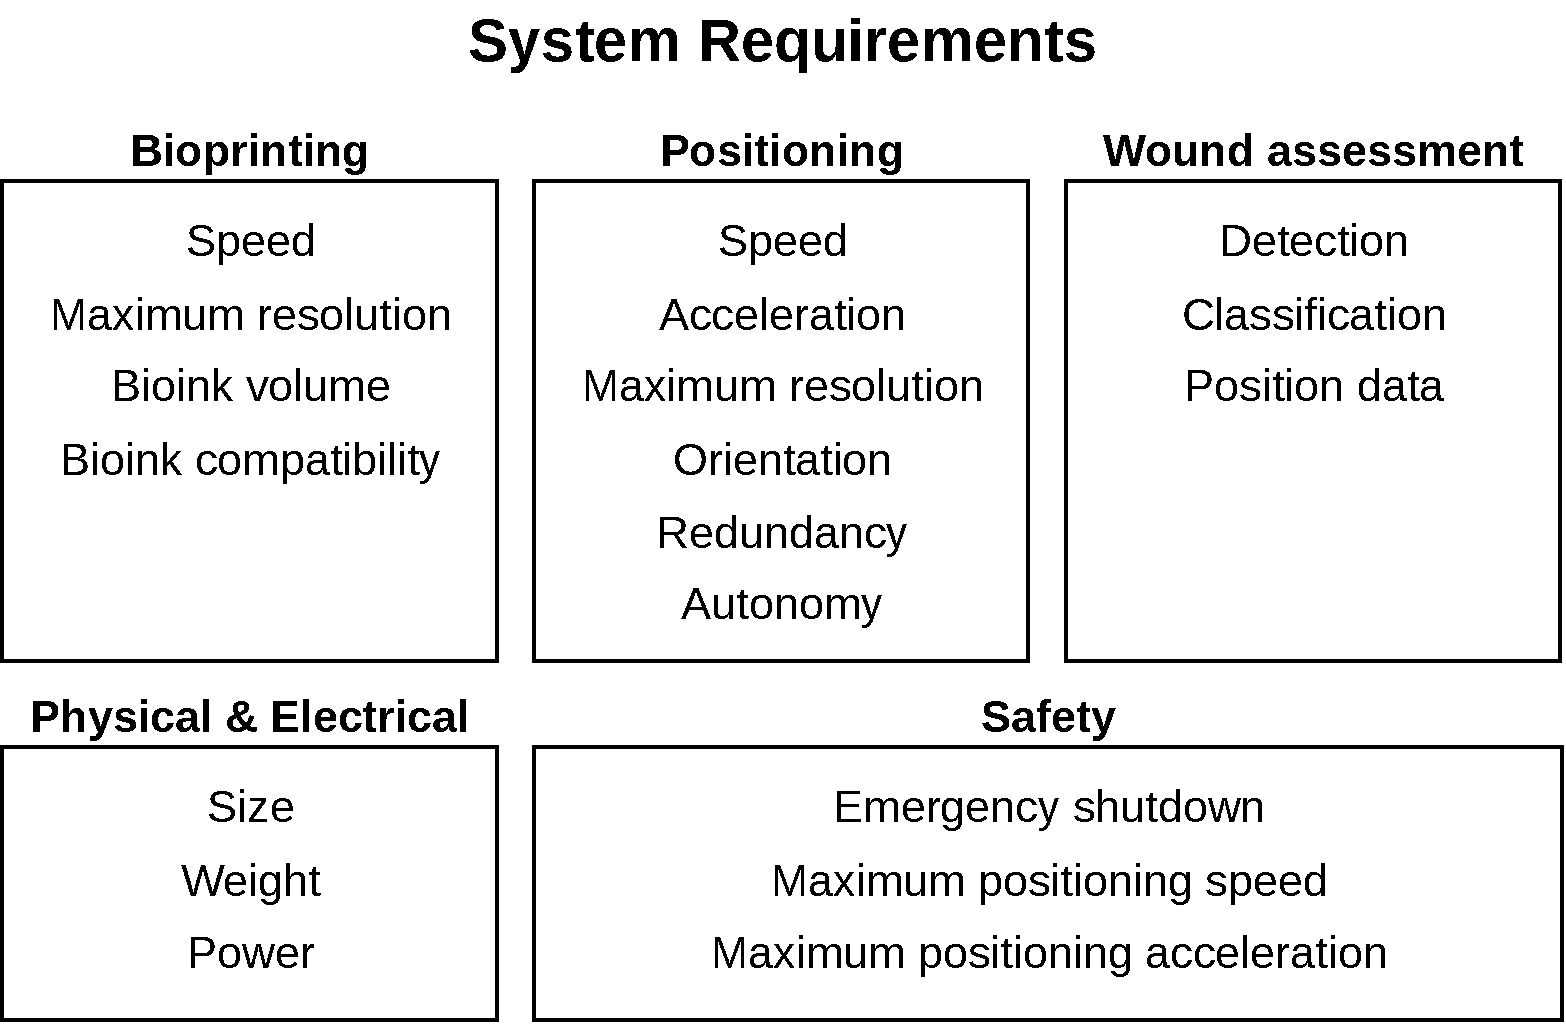
\includegraphics[width=0.7\textwidth]{system_requirements}
	\caption{System requirements.}
	\label{fig:system_requirements}
\end{figure}

\subsection{Bioprinting Speed}
\label{subsec:system_architecture_requirements_bioprinting_speed}

In order for the system to provide real clinical value it must allow the bioprinting procedure to execute at a certain speed. Because the printing will be in situ, the skin construct cannot be previously printed for later use. In order to be practical to the clinicians, the bioprinting system should execute the printing within the time frame of a wound dressing procedure, preferably in less time.

Other reasons why the printing speed may be important concern the bioink characteristics like gelation time and cell viability. The gelation time, is the time needed for the biokink to solidify. Sometimes, to reduce this time, different strategies are followed, like UV curing, depending on the bioink. The cell viability is conditioned by the speed because of induced shear stress added when trying to squeeze to cell-laden bioink out of the nozzle. 

This requirement will inevitably constrain the choice of the printing method. The choice must take into account practical operational needs and bioprinting technical needs.

According with Vijayavenkataraman \textit{et al} \cite{Vijayavenkataraman2018_bioprinting_tissues_organs_regen_med}, the slowest method seems to be the \gls{ebb}.

% subsection system_architecture_requirements_bioprinting_speed

\subsection{Bioprinting Maximum Resolution}
\label{subsec:system_architecture_requirements_bioprinting_max_resolution}

The printing resolution will condition the detail of the structures obtained, the printing speed and the resolution of the positioning system. It depends on the printing method and bioink characteristics.

Regarding the method used, the values "5, 50 and 100 \si{\micro\meter} are typically obtained by \gls{lbb}, \gls{dbb} and \gls{ebb}, respectively" \cite{Datta2018_essential_steps_bioprinting}.

{\color{red} Mostrar tabela comparativa com dados das várias características dos sistemas de bioimpressão.}

% subsection system_architecture_requirements_bioprinting_max_resolution

\subsection{Bioprinting Bioink Volume}
\label{subsec:system_architecture_requirements_bioprinting_bioink_volume}

This criteria is very important on our particular application. The print head volume will defined the amount of bioink that can be used in one go. Because we can deal with large wounds, it is important to have a good volume. If the volume is small, it may require several refills, which would affect considerably the printing time.

However, there is an upper limit based on weight, size and common wound sizes.

% subsection system_architecture_requirements_bioprinting_bioink_volume

\subsection{Bioprinting Bioink Compatibility}
\label{subsec:system_architecture_requirements_bioprinting_bioink_compatibility}

Printing skin constructs is not the same as printing bone or other organs. Bioinks for skin printing have some particular characteristics. {\color{red}Falta terminar...}

% subsection system_architecture_requirements_bioprinting_bioink_compatibility

\subsection{Positioning Speed}
\label{subsec:system_architecture_requirements_positioning_speed}

The speed of the positioning system must match the needs of the printing speed. Its maximum speed must exceed the printing speed, so that it can follow the printing process on the full range of speeds.

Since the shape of the wound can be non-planar, all the axis should be able to reach speeds greater that the maximum printing speed.

% subsection system_architecture_requirements_positioning_speed

\subsection{Positioning Acceleration}
\label{subsec:system_architecture_requirements_positioning_acceleration}

The positioning acceleration is important to guarantee that the robot can reduce its speed to zero very fast. It can also be important depending on the printing trajectories. A sudden change in direction will need a high acceleration. The positioning system must allow for high accelerations even if they are not always needed.

% subsection system_architecture_requirements_positioning_acceleration

\subsection{Positioning Maximum Resolution}
\label{subsec:system_architecture_requirements_positioning_max_resolution}

The maximum resolution of the positioning system is the minimum repeatable step size. This will define the precision of the system. It is very important that this value is lower than the bioprinting resolution, by at least one order of magnitude. In case this is not possible, the printing method must be adapted to accommodate for this limitation and still be effective.

Gantry systems can have very high resolutions. That is one of the reasons they are so often used in 3D printing and bioprinting. Other robotic manipulators on the other hand, can have many degrees of freedom, but typically lose resolution because of that.

% subsection system_architecture_requirements_positioning_max_resolution

\subsection{Positioning Orientation}
\label{subsec:system_architecture_requirements_positioning_orientation}

For this specific application, the print head orientation is very relevant. We have to consider a system that must be able to print on a wound that is located anywhere in the body. To be more practical it would also be ideal for the system to move according to the patient position instead of the other way around. Because of this, the print head may need to work in various non vertical orientations.

Gantry systems have the limitation of having a fixed orientation. Robotic manipulators with more degrees of freedom can have partial or full orientation freedom.

% subsection system_architecture_requirements_positioning_orientation

\subsection{Positioning Redundancy}
\label{subsec:system_architecture_requirements_positioning_redundancy}

Another important aspect of positioning is redundancy. This means having extra degrees of freedom to handle obstacles, for example. These extra \gls{dof} for a specific task allows the system to position the print head on one place with different configurations. The facilitates the process of the system adapting to the patient vs the patient adapting to the system.

% subsection system_architecture_requirements_positioning_redundancy

\subsection{Positioning Autonomy}
\label{subsec:system_architecture_requirements_positioning_autonomy}

The degree of autonomy of the positioning system must also be considered. The system may be fully autonomous using sensing data to detect the wound, position itself along it, and execute the printing. But it can also work semi-autonomously, where the clinician manipulates the system as a tool and controls the printing directly. The positioning system only provides some extra control on the procedure.

% subsection system_architecture_requirements_positioning_autonomy

\subsection{Wound Assessment Detection}
\label{subsec:system_architecture_requirements_wound_assessment_detection}

Since the goal is to print directly on a wound, the system must be able to detect the wound. This detection can be operator dependent, i.e., the operator guides the positioning system towards the wound area. Another possibility is to use a sensing system to detect the wound and guide the positioning system. It is somewhat related to the positioning autonomy.

The are several possibilities for this wound detection as was shown on chapter \ref{cha:literature_review}.

% subsection system_architecture_requirements_wound_assessment_detection

\subsection{Wound Assessment Classification}
\label{subsec:system_architecture_requirements_wound_assessment_classification}

Wound classification is the action of extracting meaningful data after detection. Some important data to support the autonomy of the printing process is measuring the wound area and perimeter. Other important parameters may be the depth and profile.

The wound area is important to calculate the amount of bioink needed for the print. It also can help the clinicians in assessing the \gls{tbsa}. 

% subsection system_architecture_requirements_wound_assessment_classification

\subsection{Wound Assessment Position Data}
\label{subsec:system_architecture_requirements_wound_assessment_position_sharing}

After wound detection by a sensing system, the wound position must be shared with the positioning system for the printing to occur on the right place. The data sharing process and the data itself must be considered. It will depend on the sensing system, but at least a reference transformation between the sensing system and the positioning system must exist.

% subsection system_architecture_requirements_wound_assessment_position_sharing

\subsection{Physical Size}
\label{subsec:system_architecture_requirements_physical_size}

As in all physical products, the size is always something to consider. The system will be installed on a operating room or a patient room, which are not huge and many times already crowded with other tools and machines. So, in this case, the whole system should not be too big.

It should occupy the least space possible, but still have enough range to reach the patients vertical axis (central line) from the patient's side.

% subsection system_architecture_requirements_physical_size

\subsection{Physical Weight}
\label{subsec:system_architecture_requirements_physical_mass}

The system's mass is also important. It should weight as less as possible. One specific reason for this is for safety. Since the positioning system maybe working autonomously close to the patient, it is vital to have a reduced mass in case of contact. 

Another reason is for manipulation. If the system is to be manipulated directly by an operator for the bioprinting procedure, it facilitates if it is low weight. The system must help the clinicians, not introduce more hurdles.

The mass also interferes with the degree of portability of the system. It if it is light, it can be moved between difference spaces easily. This facilitates the process of taking the system to where it is needed.

% subsection system_architecture_requirements_physical_mass

\subsection{Electrical Power}
\label{subsec:system_architecture_requirements_physical_power}

The power here considered is electrical power. If the system can use the normal mains power to operate it does not need a special installation. This will help cut down costs and ease the installation. If the system was three-phase, for example, the electrical system on the room would need to be updated.

% subsection system_architecture_requirements_physical_power

\subsection{Safety Emergency Shutdown}
\label{subsec:system_architecture_requirements_safety_emergency_shutdown}

For safety considerations, an emergency shutdown must be considered. The system will be in almost direct contact with the patient during printing. If something goes wrong, there must exist a way to turn off the system to prevent any or further injuries, to the patient or operator.

% subsection system_architecture_requirements_safety_emergency_shutdown

\subsection{Safety Maximum Positioning Speed}
\label{subsec:system_architecture_requirements_safety_max_positioning_speed}

Although having a fast positioning system is good, a maximum limit must exists that minimises the change of injury if an accidental contact between a person and the system occurs.

% subsection system_architecture_requirements_safety_max_positioning_speed

\subsection{Safety Maximum Positioning Acceleration}
\label{subsec:system_architecture_requirements_safety_max_positioning_acceleration}

Regarding the acceleration, there must be a maximum limit, as with speed, to prevent any injuries or minimise the consequences of one. Since a human and a robot will be working on the same space, any safety measure available must be considered.

% subsection system_architecture_requirements_safety_max_positioning_acceleration

% section system_architecture_requirements

% ==========================
% = System Components =
% ==========================

\section{System Components}
\label{sec:system_architecture_components}

Based on the system requirements previously mentioned, the system suggested is composed by three main components (Fig. \ref{fig:system_architecture_components}): (a) a robotic system composed by a robotic manipulator that is responsible for positioning the print head in space; (b) a vision system responsible for wound assessment; and (c) a bioprinting system composed by a extrusion-based print head.

\begin{figure}[htbp]
	\centering
	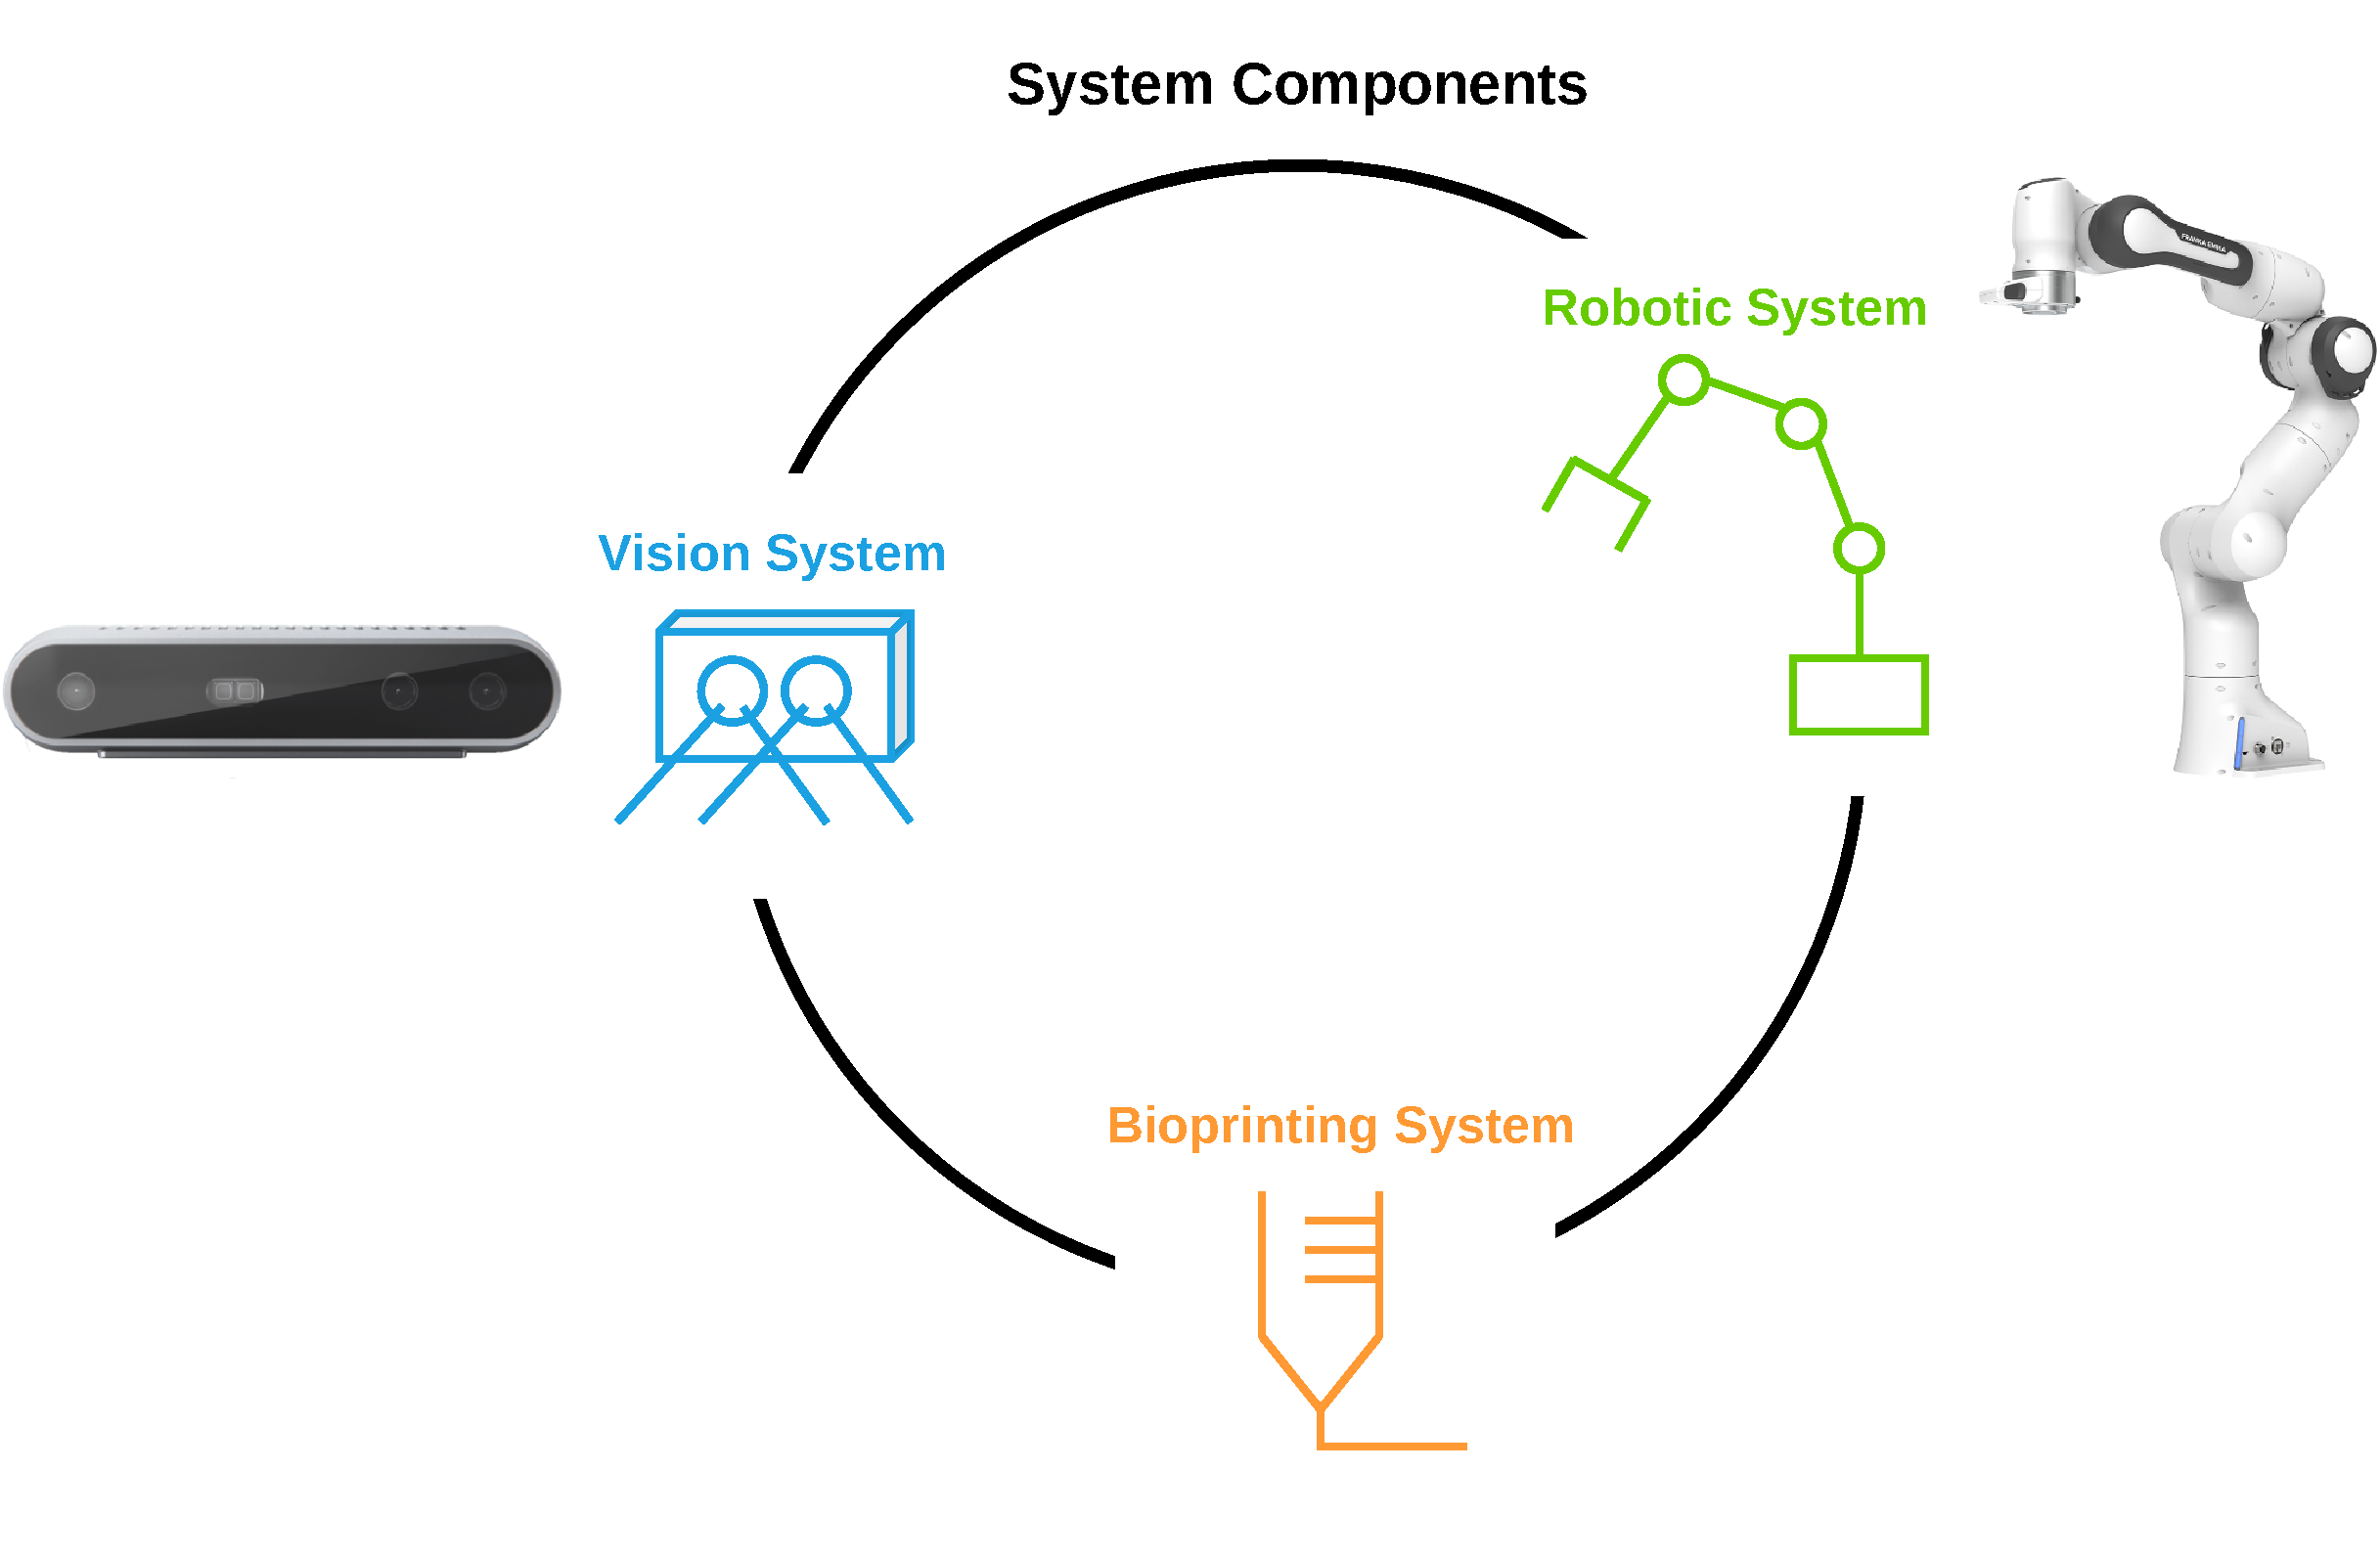
\includegraphics[width=.6\textwidth]{system_architecture_components_complete}
	\caption{System architecture main components. The robotic system is a Panda 7 \gls{dof} robotic manipulator. The vision system is an Intel\textregistered RealSense\texttrademark{} D415 depth camera. The bioprinting system consists of a custom made syringe pump print head.}
	\label{fig:system_architecture_components}
\end{figure}

\subsection*{Robotic System}
\label{subsec:system_architecture_components_robotic_system}

The robotic system consists in a 7 \gls{dof} robotic manipulator. Position redundancy and orientation requirements are naturally satisfied. By having seven degrees of freedom this robot is inherently redundant for any task in 3D space.

To fully describe an object in space, at least six degrees of freedom are need. Three degrees define the position, i.e., the x, y and z coordinates in relation to a reference frame. The other three degrees define the orientation. For example, the three Euler angles ($\alpha, \beta, \gamma$) suffice for orientation definition.

In terms of resolution, this robotic manipulator guarantees 100 \si{\micro\meter}. It means it matches the normal resolution of extrusion-based bioprinting methods. {\color{red}Reference for robot datasheet.}

{\color{red} Ver referências. Falar do peso, tamanho e alimentação.}

The robotic system is thoroughly described on chapter \ref{cha:robotic_system}
.

% subsection system_architecture_components_robotic_system

\subsection*{Vision System}
\label{subsec:system_architecture_components_vision_system}

An Intel\textregistered RealSense\texttrademark{} D415 depth camera was used as the vision system. Being a depth camera, it provides not only \gls{rgb} data but also depth data.

With \gls{rgb} data, the system is able to apply computer vision algorithms to that data in order to detect a wound within the camera \gls{fov}. If we only used an \gls{rgb} camera, it would only be possible to get information about the wound position in 2D space. That is why the depth functionality comes into play.

The depth sensors will allow the detection of the distance of each pixel in relation to the camera reference frame. With that, a full 3D position in space can be obtained. This means the wound classification requirements are satisfied. 

The other positive aspect of having depth data is that we can generate point clouds out of it. With a point cloud, we can create meshes of the surfaces detected and do some form of geometric analysis.

{\color{red} Ver referências...}

The vision system is thoroughly described on chapter \ref{cha:vision_system}
.

% subsection system_architecture_components_vision_system

\subsection*{Bioprinting System}
\label{subsec:system_architecture_components_bioprinting_system}

The bioprinting system consists on a custom made robot end-effector which works as an extrusion-based print head. The concept is based on a syringe pump mechanism. Several open source/hardware projects served as inspiration for the design of the system.

The \gls{ebb} method was chosen, because it offers the best scalability at this point. Although the resolution is the worst among the three methods, our particular application does not really need better resolution. Besides, its resolution is closer to that of the robotic system. Finally, it is the easiest and cheapest method to build.

Regarding some of the requirements, the extrusion-based systems allows us to use big volume containers; have a wide diversity of compatible bioinks for various tissue constructs; and still guarantee a fairly good printing speed.

This system was developed more to provide comparable data of the bioprinting process, than really to present an innovative extrusion-based print head.

{\color{red} Ver referências...}

The vision system is thoroughly described on chapter \ref{cha:bioprinting_system}

% subsection system_architecture_components_robotic_system

% section system_architecture_components
.
% ==========================
% = Functional Diagrams =
% ==========================

\section{Functional Diagrams}
\label{sec:system_architecture_functional_diagrams}

At this point it is important to understand how the system components interact with each other. A set of functional diagrams show this interaction, i.e., how the components communicate to exchange data and commands to attain the final goal of a working system.

Figure \ref{fig:system_architecture_functional_diagram_overview} presents an overview of the main components interactions. Each of the main components, robotic, vision, and bioprinting systems communicate to a central control system. This central control system is a computer that runs the software application which communicates with the other systems.

\begin{figure}[htbp]
	\centering
	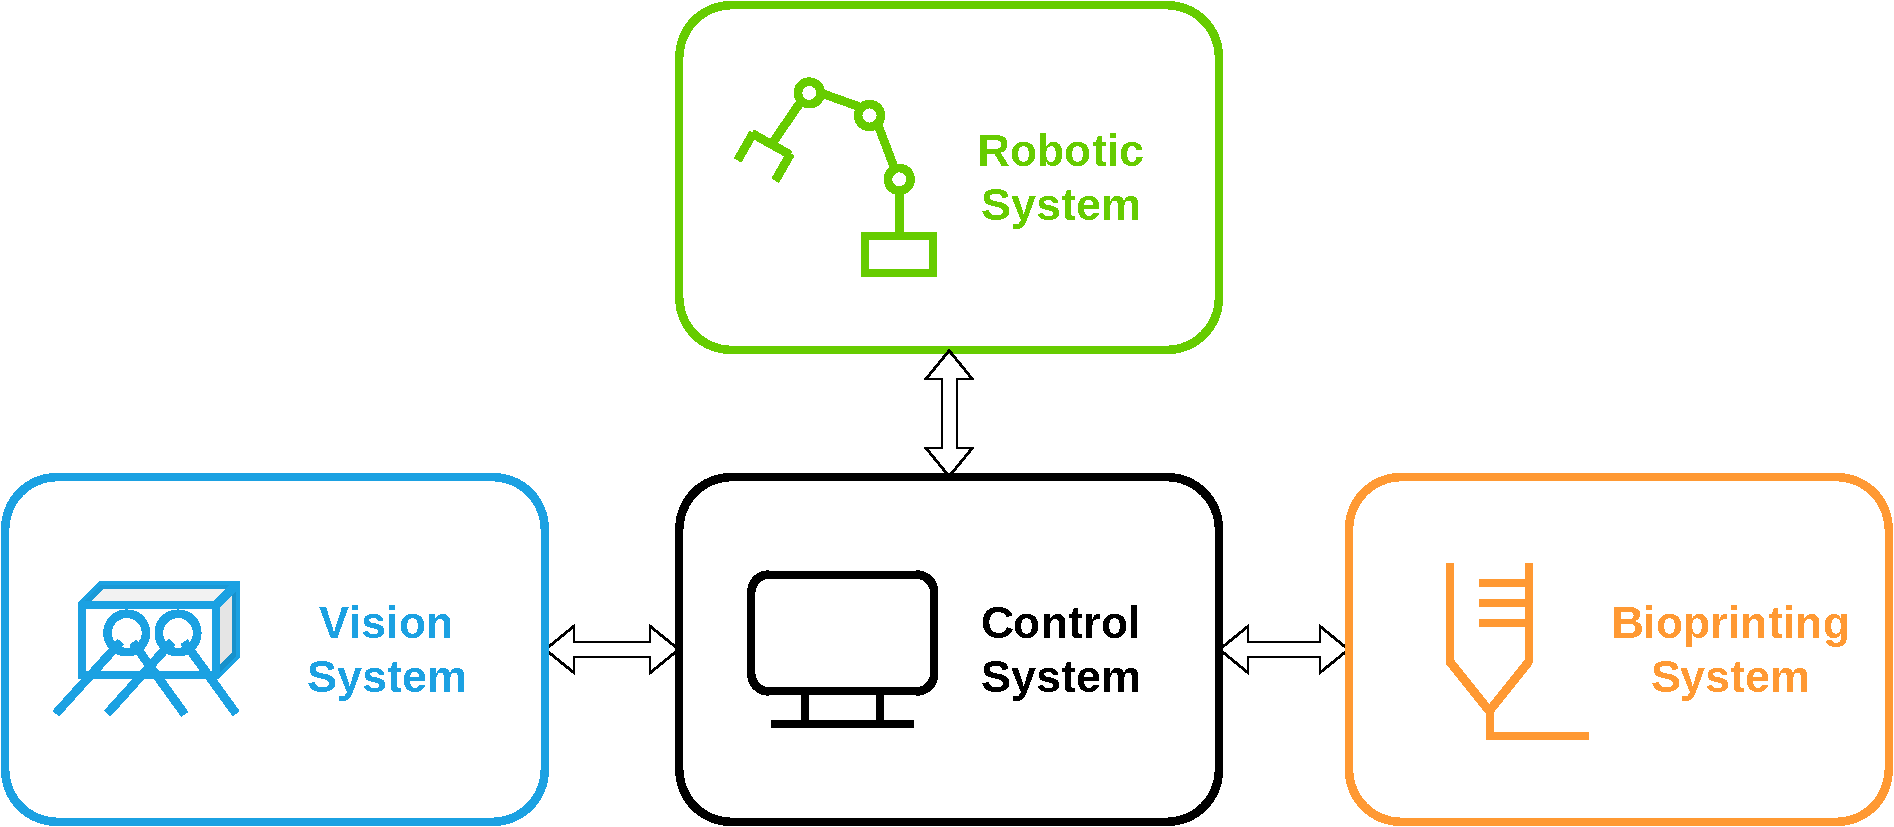
\includegraphics[width=\textwidth]{system_architecture_functional_diagram_overview}
	\caption{System architecture functional diagram overview. It shows the communication interaction between the different components.}
	\label{fig:system_architecture_functional_diagram_overview}
\end{figure}

The robotic, vision, and bioprinting systems, are basically hardware and firmware/software the control the systems themselves and define the communication protocols and data exchange.\\

The robotic system has to main pieces of hardware. The robotic arm and a control unit. They communicate with each other by a proprietary protocol. The robotic arm is mainly hardware and firmware. The control unit is a computer itself running an operating system and control software (Fig. \ref{fig:system_architecture_functional_diagram_robotic_system}).

The control system communicates with the robotic system via the robotic system's control unit through the Ethernet protocol, exchanging control commands and kinematics/dynamics data (Fig. \ref{fig:system_architecture_functional_diagram_robotic_system}).

The robotic system internal architecture is the manufacturer's responsibility. More detailed information on this system is provided on chapter \ref{cha:robotic_system}.

\begin{figure}[htbp]
	\centering
	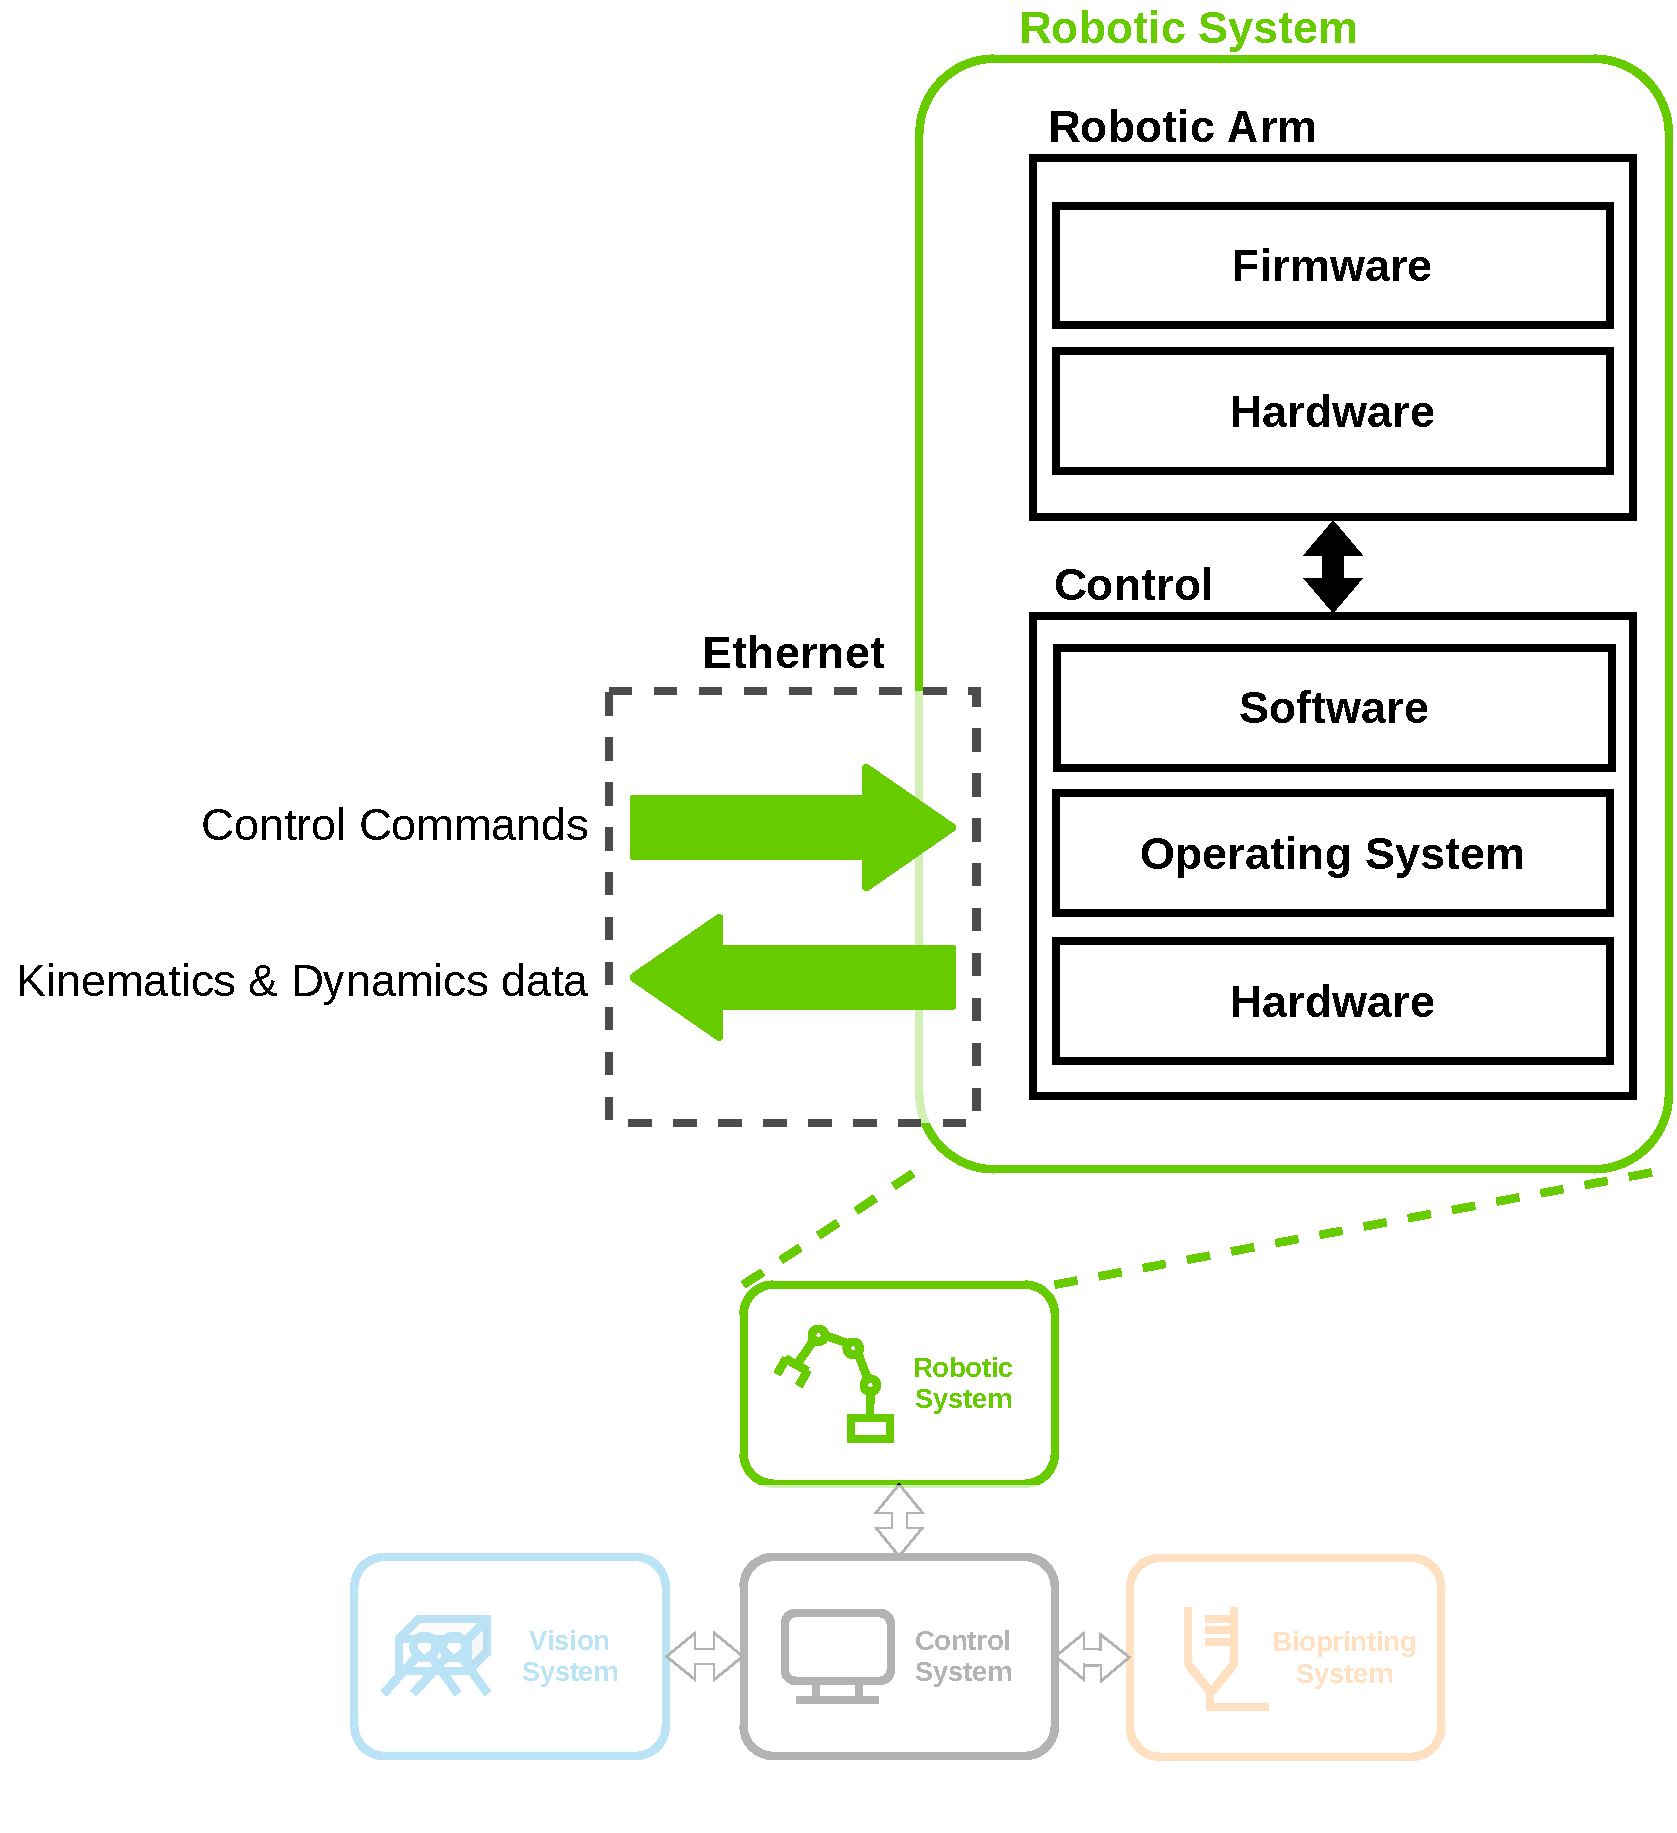
\includegraphics[width=0.6\textwidth]{system_architecture_functional_diagram_robotic_system}
	\caption{System architecture functional diagram of the robotic system. The robotic system is made of two hardware parts that communicate with each other. The global control system communicates with the robotic system via the robotic system's control unit using the Ethernet protocol.}
	\label{fig:system_architecture_functional_diagram_robotic_system}
\end{figure}

The vision and bioprinting systems have a similar internal architecture. The vision system consists on the depth camera composed by an hardware layer and a firmware layer (Fig. \ref{fig:system_architecture_functional_diagram_vision_bioprinting_system} (left)). The latter controls the hardware and implements the communication protocol via \gls{usb}. The whole architecture was developed by the manufacturer.

For a more detailed description of the vision system, refer to chapter \ref{cha:vision_system}.\\

The bioprinting system, as previously mentioned, consists on a custom made print head. Its architecture, the hardware and firmware layers were developed on this thesis. The communication interface used was also \gls{usb}. The communication \gls{api} allows the control system to inquiry about the available bioink volume and send commands to control the bioink dispensing (Fig. \ref{fig:system_architecture_functional_diagram_vision_bioprinting_system} (right)).

For the complete description of the bioprinting system, refer to chapter \ref{cha:bioprinting_system}.

\begin{figure}[htbp]
	\centering
	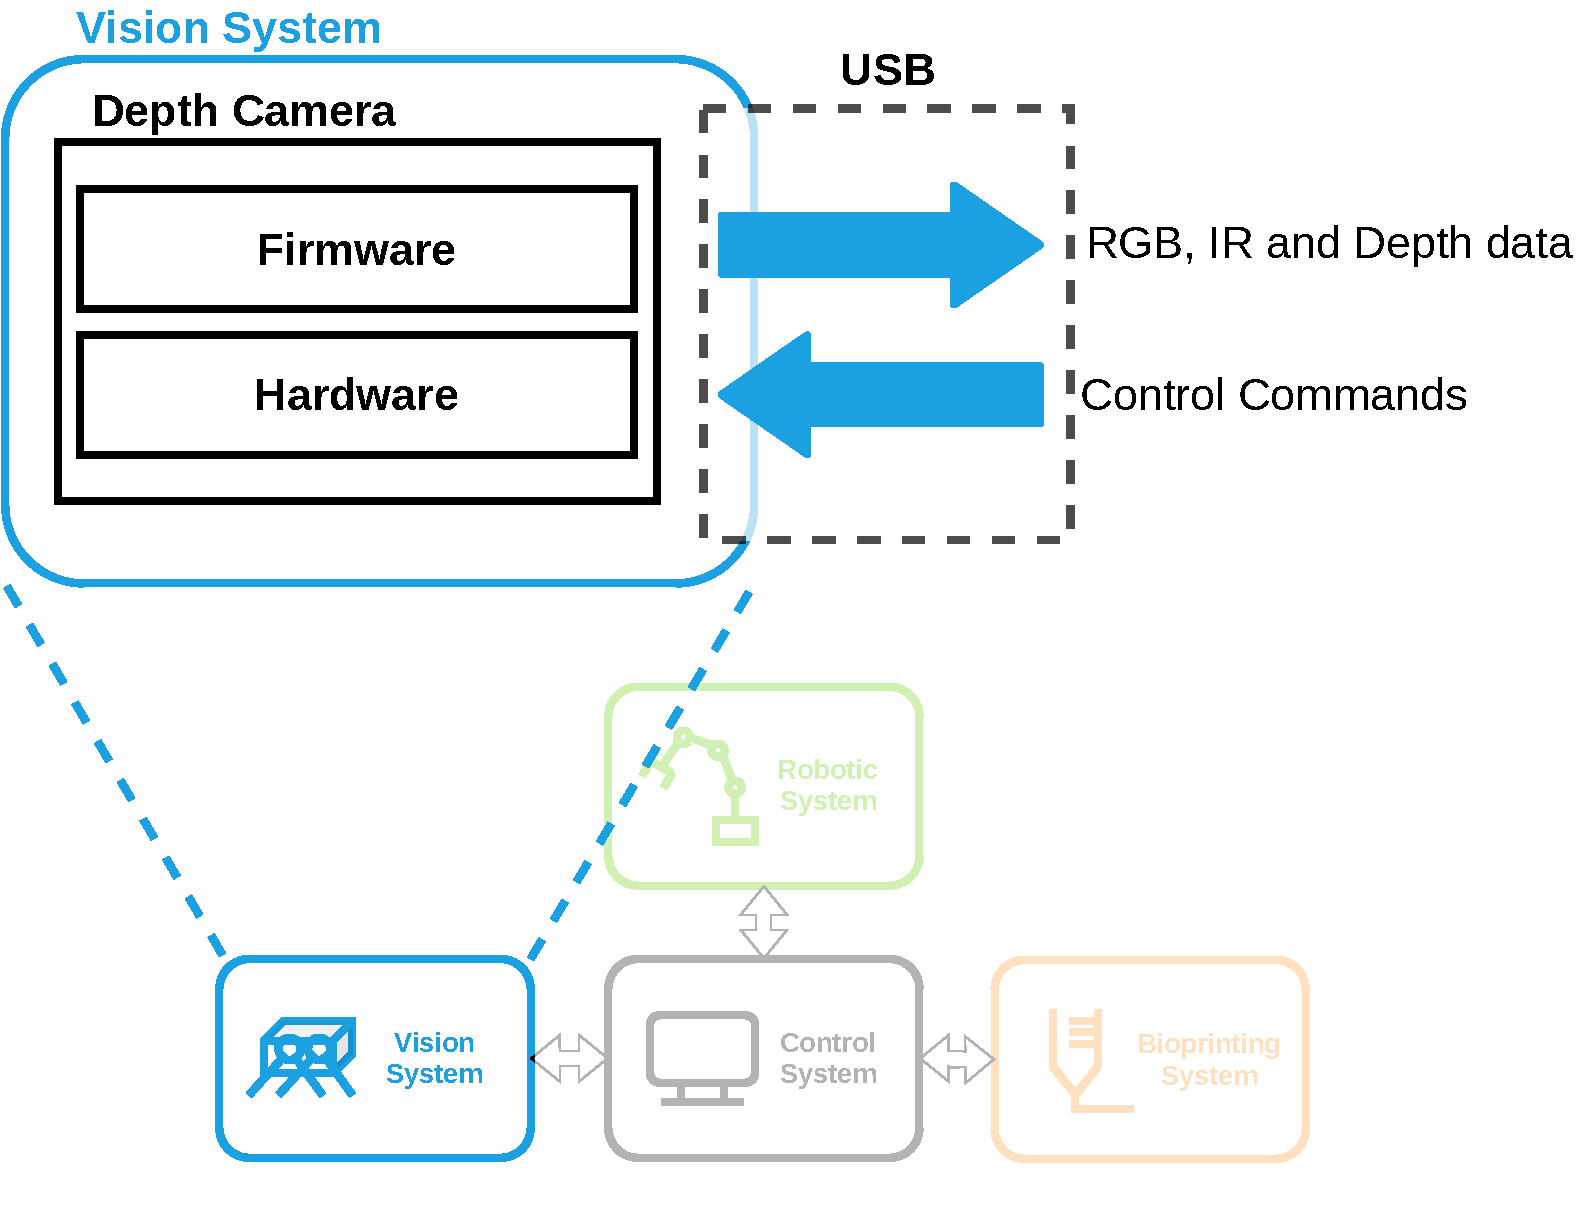
\includegraphics[width=0.45\textwidth]{system_architecture_functional_diagram_vision_system}
	\hspace{0.1in}
	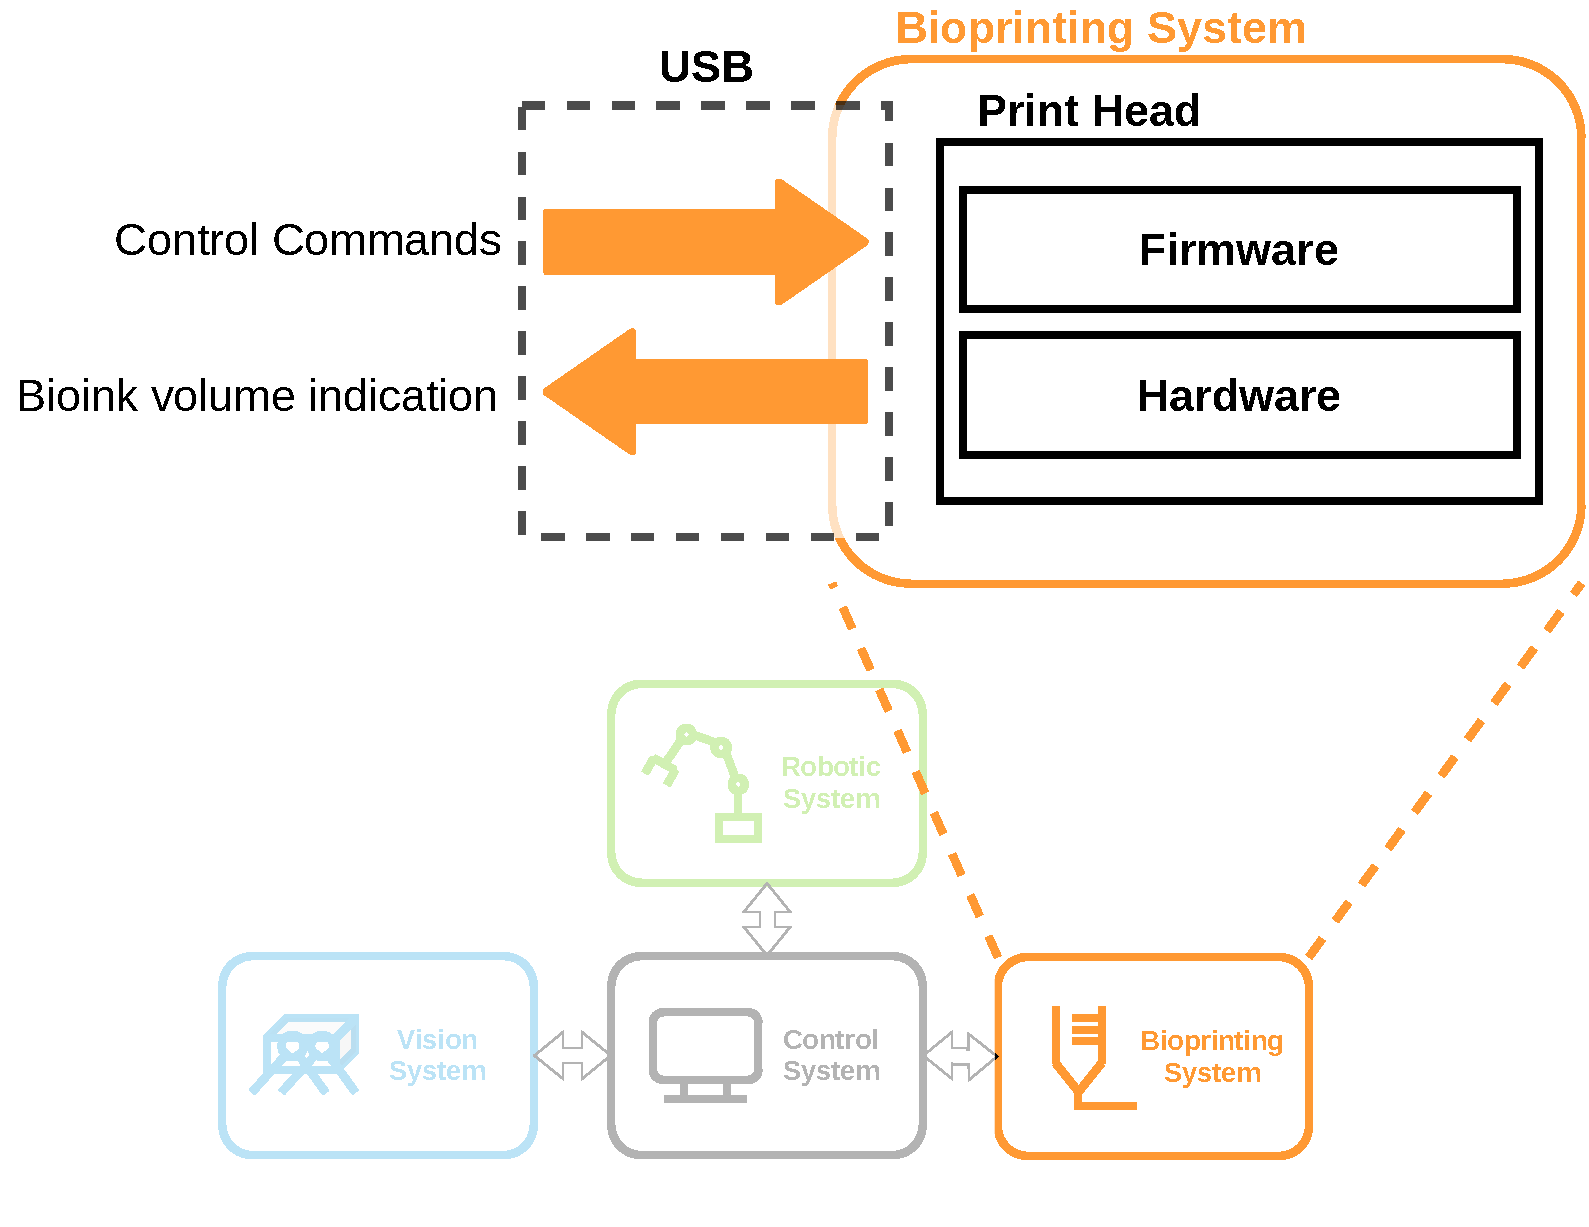
\includegraphics[width=0.45\textwidth]{system_architecture_functional_diagram_bioprinting_system}
	\caption{System architecture functional diagrams of the vision (left) and bioprinting (right) systems. Both systems share a similar architecture. They have only hardware and firmware layers. The vision system architecture is manufacturer dependent, and the bioprinting was custom made within this thesis work.}
	\label{fig:system_architecture_functional_diagram_vision_bioprinting_system}
\end{figure}

Finally, the control system's architecture consists on several layers like: (a) the common layers of a personal computer, the hardware and operating system layers; (b) a middle-ware layer, \gls{ros}; and (c) an application layer, which consists on the main work of this thesis (Fig. \ref{fig:system_architecture_functional_diagram_control_system}).

The application layer was built directly on top of \gls{ros} which means it is completely dependent on its existence. The reason this is done this way is because both the robot and the camera have \gls{ros} integrations. Besides, \gls{ros} uses a distributed architecture that eases the communication between the different nodes. A detailed description of \gls{ros} is provided on Annex \ref{ann:ros}.

The application itself is composed of several layers, each belonging to a specific system (Fig. \ref{fig:system_architecture_functional_diagram_control_system}). In operational terms, they all stack up, like shown on Figure \ref{fig:system_architecture_intro} (right), passing data to the top adjacent layer. Some layers belong to the same \gls{ros} package and can even belong to the same node. In general, a system is represented by a package but not necessarily.

\begin{figure}[htbp]
	\centering
	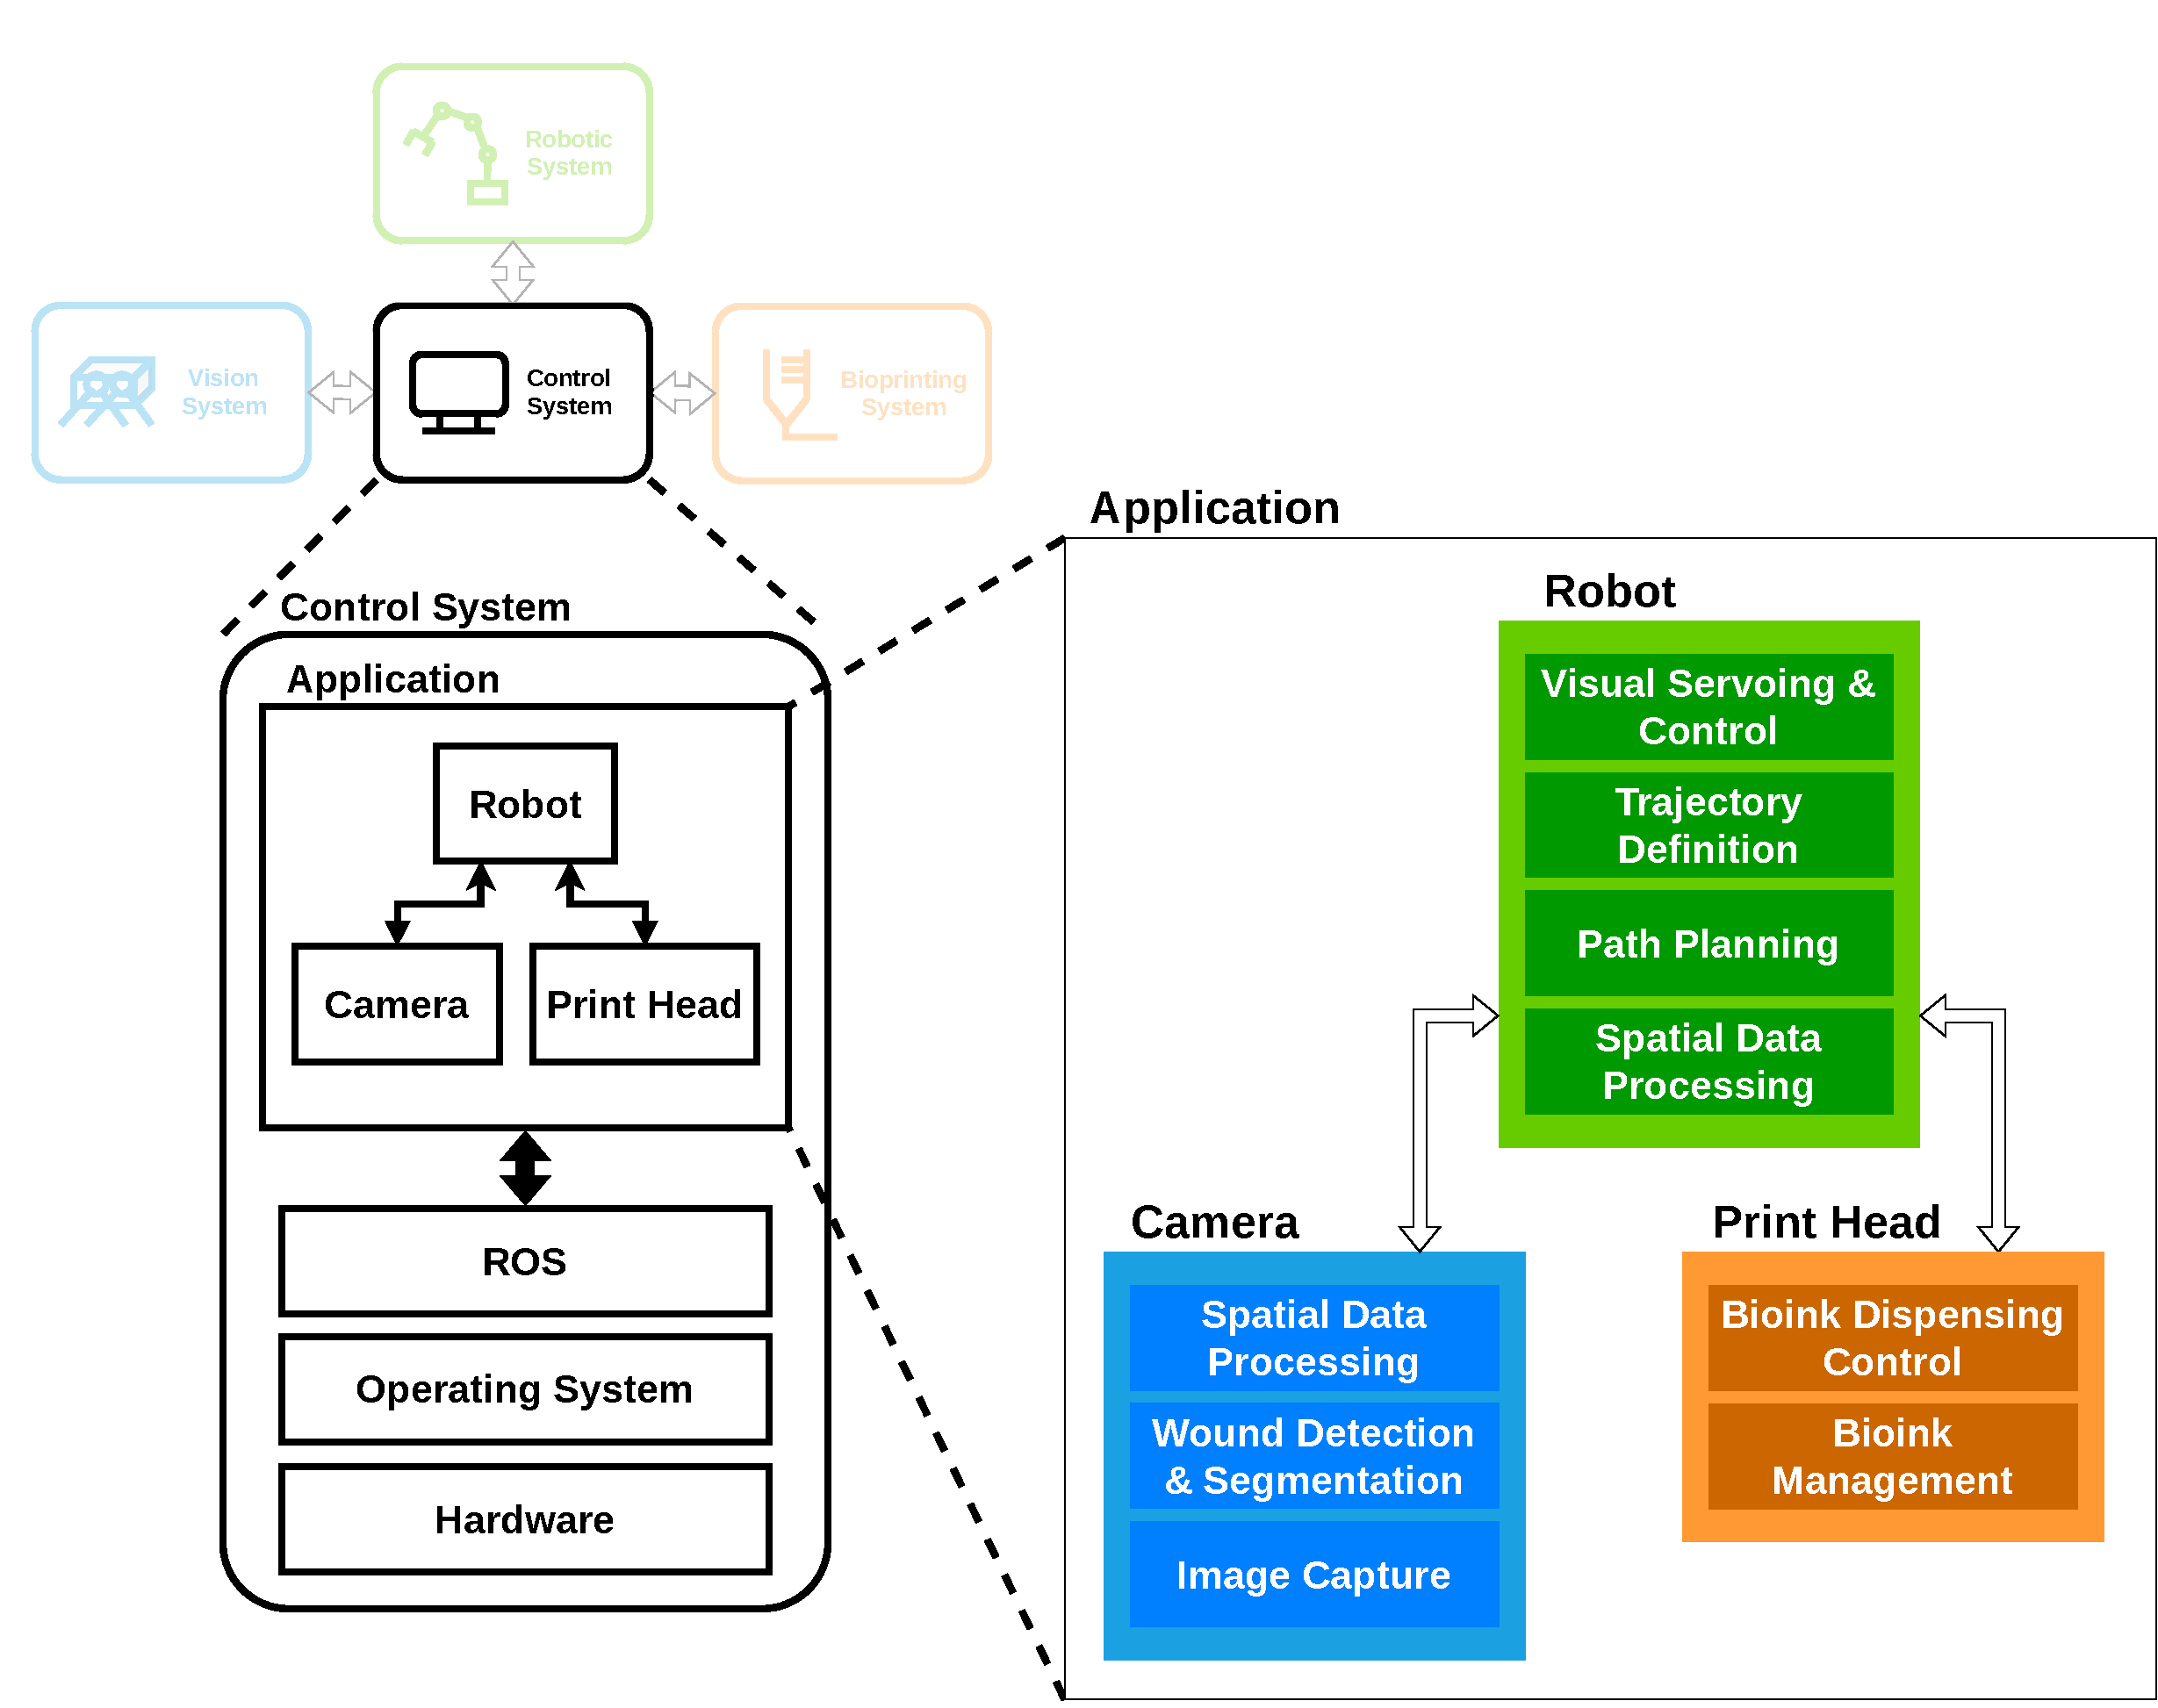
\includegraphics[width=0.9\textwidth]{system_architecture_functional_diagram_control_system}
	\caption{System architecture functional diagram overview.}
	\label{fig:system_architecture_functional_diagram_control_system}
\end{figure}

Each layer is documented in detail on section \ref{sec:system_architectural_layers}.

% section system_architecture_functional_diagrams

% ==========================
% = Architectural Layers =
% ==========================

\section{Architectural Layers}
\label{sec:system_architectural_layers}

Nine layers compose the control system application. Next, they will be thoroughly described. Figure \ref{fig:system_architecture_layers_detail} presents a more detailed view of the layers composition and inter-layer communication.

\begin{figure}[htbp]
	\centering
	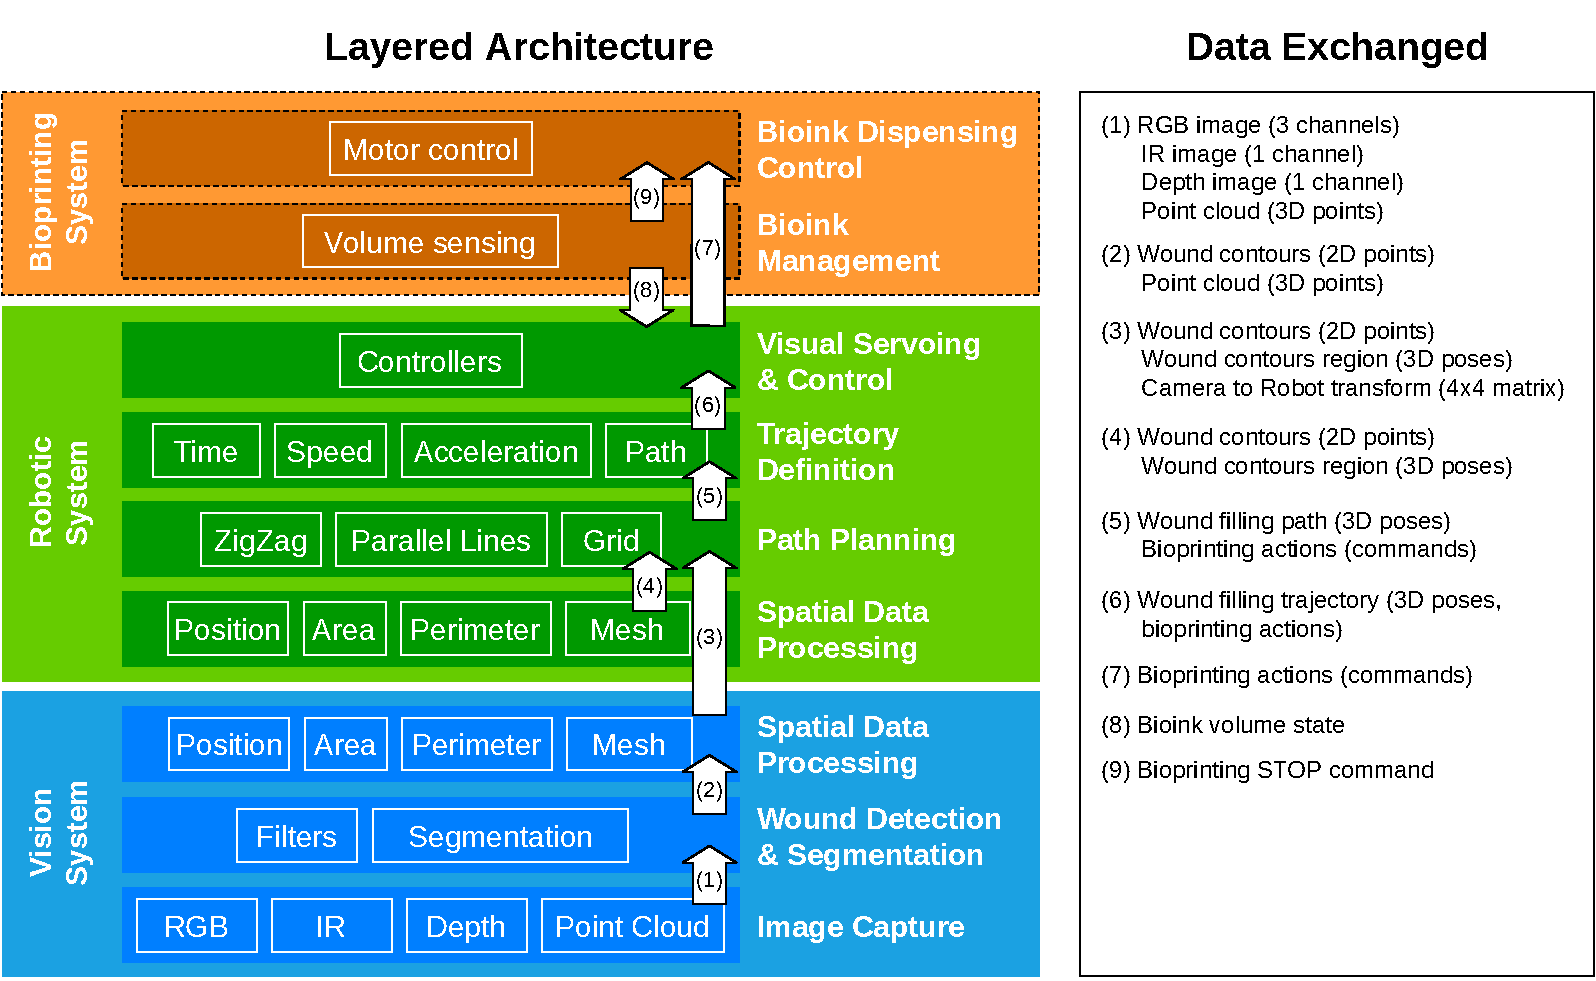
\includegraphics[width=\textwidth]{system_architecture_layers_detail}
	\caption{System's architectural layers detail. Each layer shows their internal blocks which corresponds to the data gathered or the type of actions taken on that layer. The arrows represent the inter-layer interaction. On the \textit{Data Exchanged} area the data types that are exchanged between layers are listed. }
	\label{fig:system_architecture_layers_detail}
\end{figure}

\subsection{Camera Layers}
\label{subsec:system_architectural_camera_layers}

The camera layers are responsible for obtaining wound data out of the camera image stream. That data will then be used by the robot arm to guide the print head through the wound filling bioprinting procedure.

\subsubsection*{Image Capture}
\label{subsubsec:system_architectural_camera_layers_image_capture}

This layer is responsible for tapping into the camera image stream. Figure \ref{fig:system_architecture_layer_image_capture_flowchart} presents the flowchart of this layer.

\begin{figure}[htbp]
	\centering
	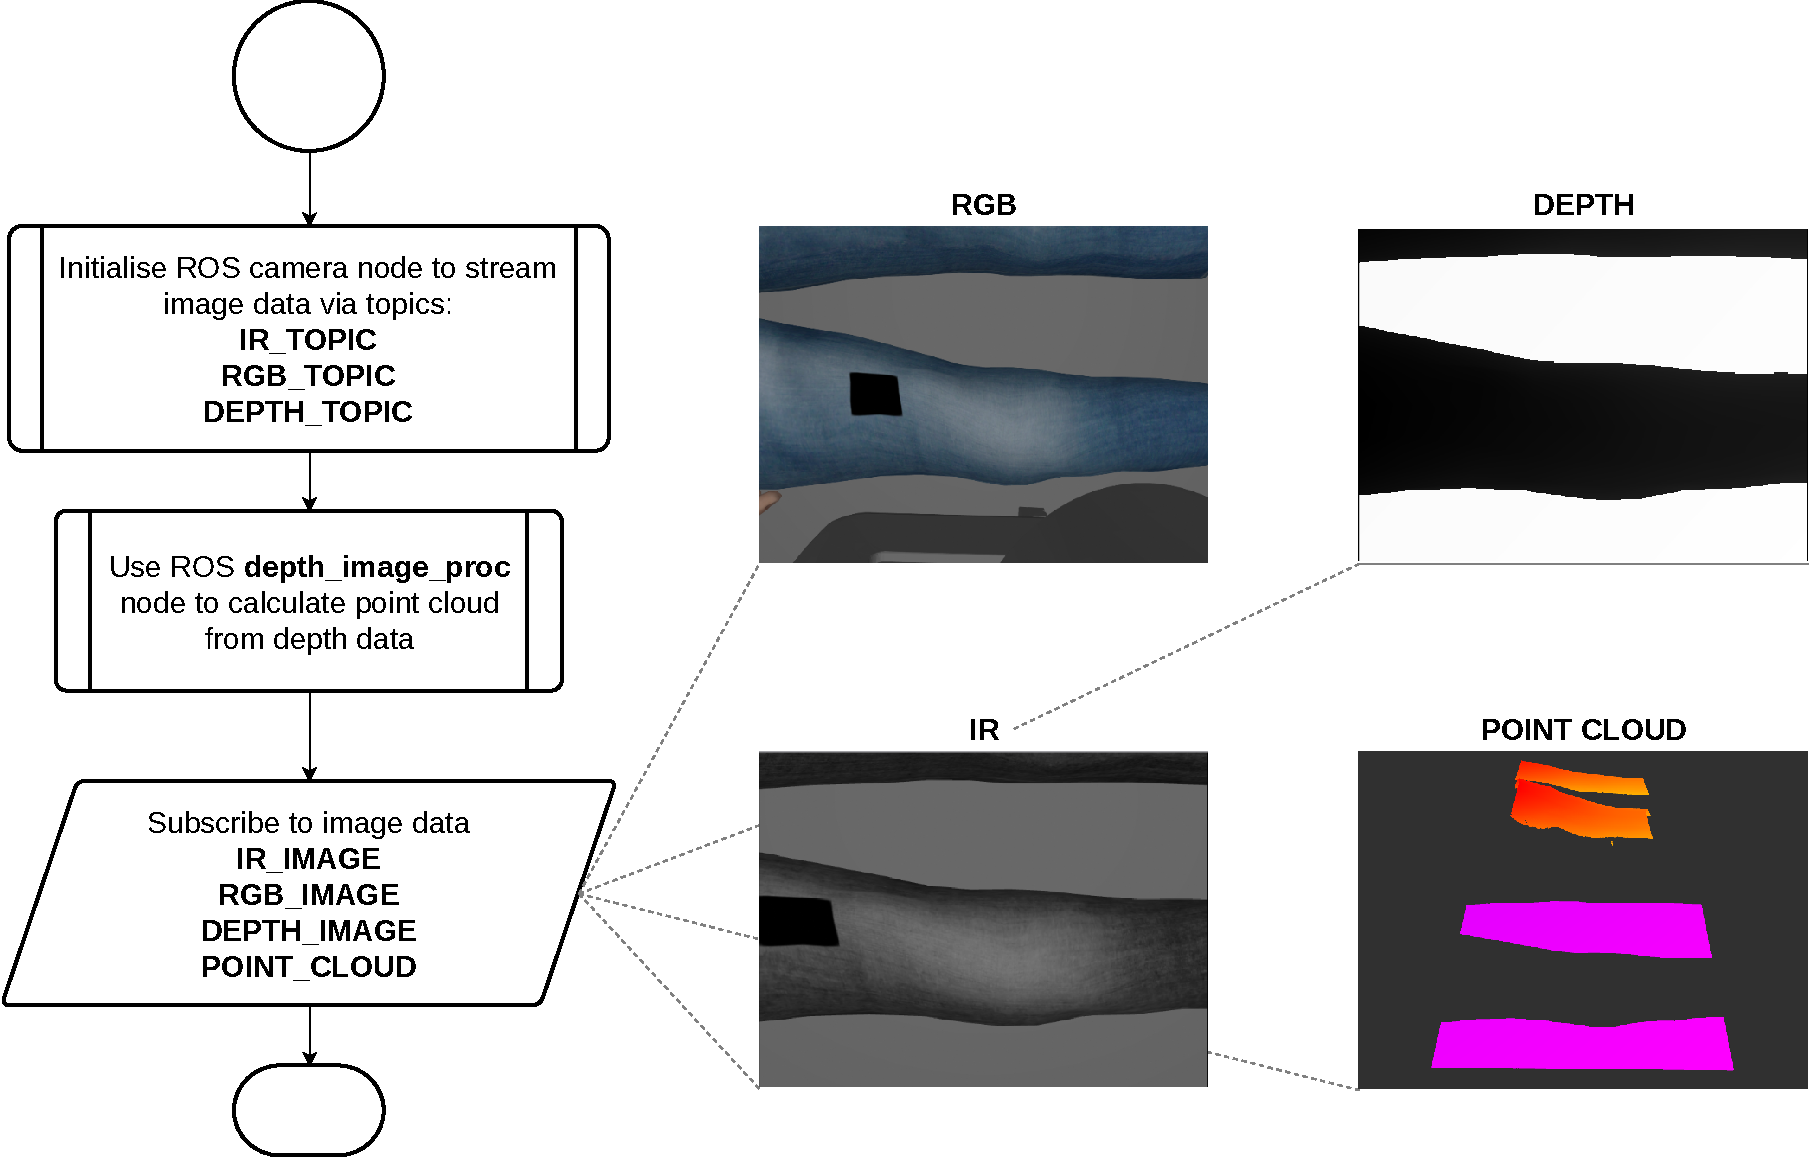
\includegraphics[width=\textwidth]{system_architecture_layer_image_capture_flowchart}
	\caption{sdfsfsfsfsd}
	\label{fig:system_architecture_layer_image_capture_flowchart}
\end{figure}

{\color{red}Explain the flowchart.}

% subsubsection system_architectural_camera_layers_image_capture

\subsubsection*{Wound Detection \& Segmentation}
\label{subsubsec:system_architectural_camera_layers_wound_detection_segmentation}

The wound detection \& segmentation layer is probably the most important layer associated with the camera. At this level is where the camera becomes really useful and fullfils its purpose, which is detecting the a burn wound on its \gls{fov}.

As discussed on section \ref{sec:burn_wound_segmentation} there are many different algorithms, with different complexities and outcomes, for wound detection. On this work, for the sake of simplicity and developing the whole chain, a very simplistic approach was followed.

The wound model consists of a simple shape painted black. This allows for a very simple binarization approach to be used. Figure \ref{fig:system_architecture_layer_wound_detection_segmentation_flowchart} presents the flowchart of wound detection and segmentation.

\begin{figure}[htbp]
	\centering
	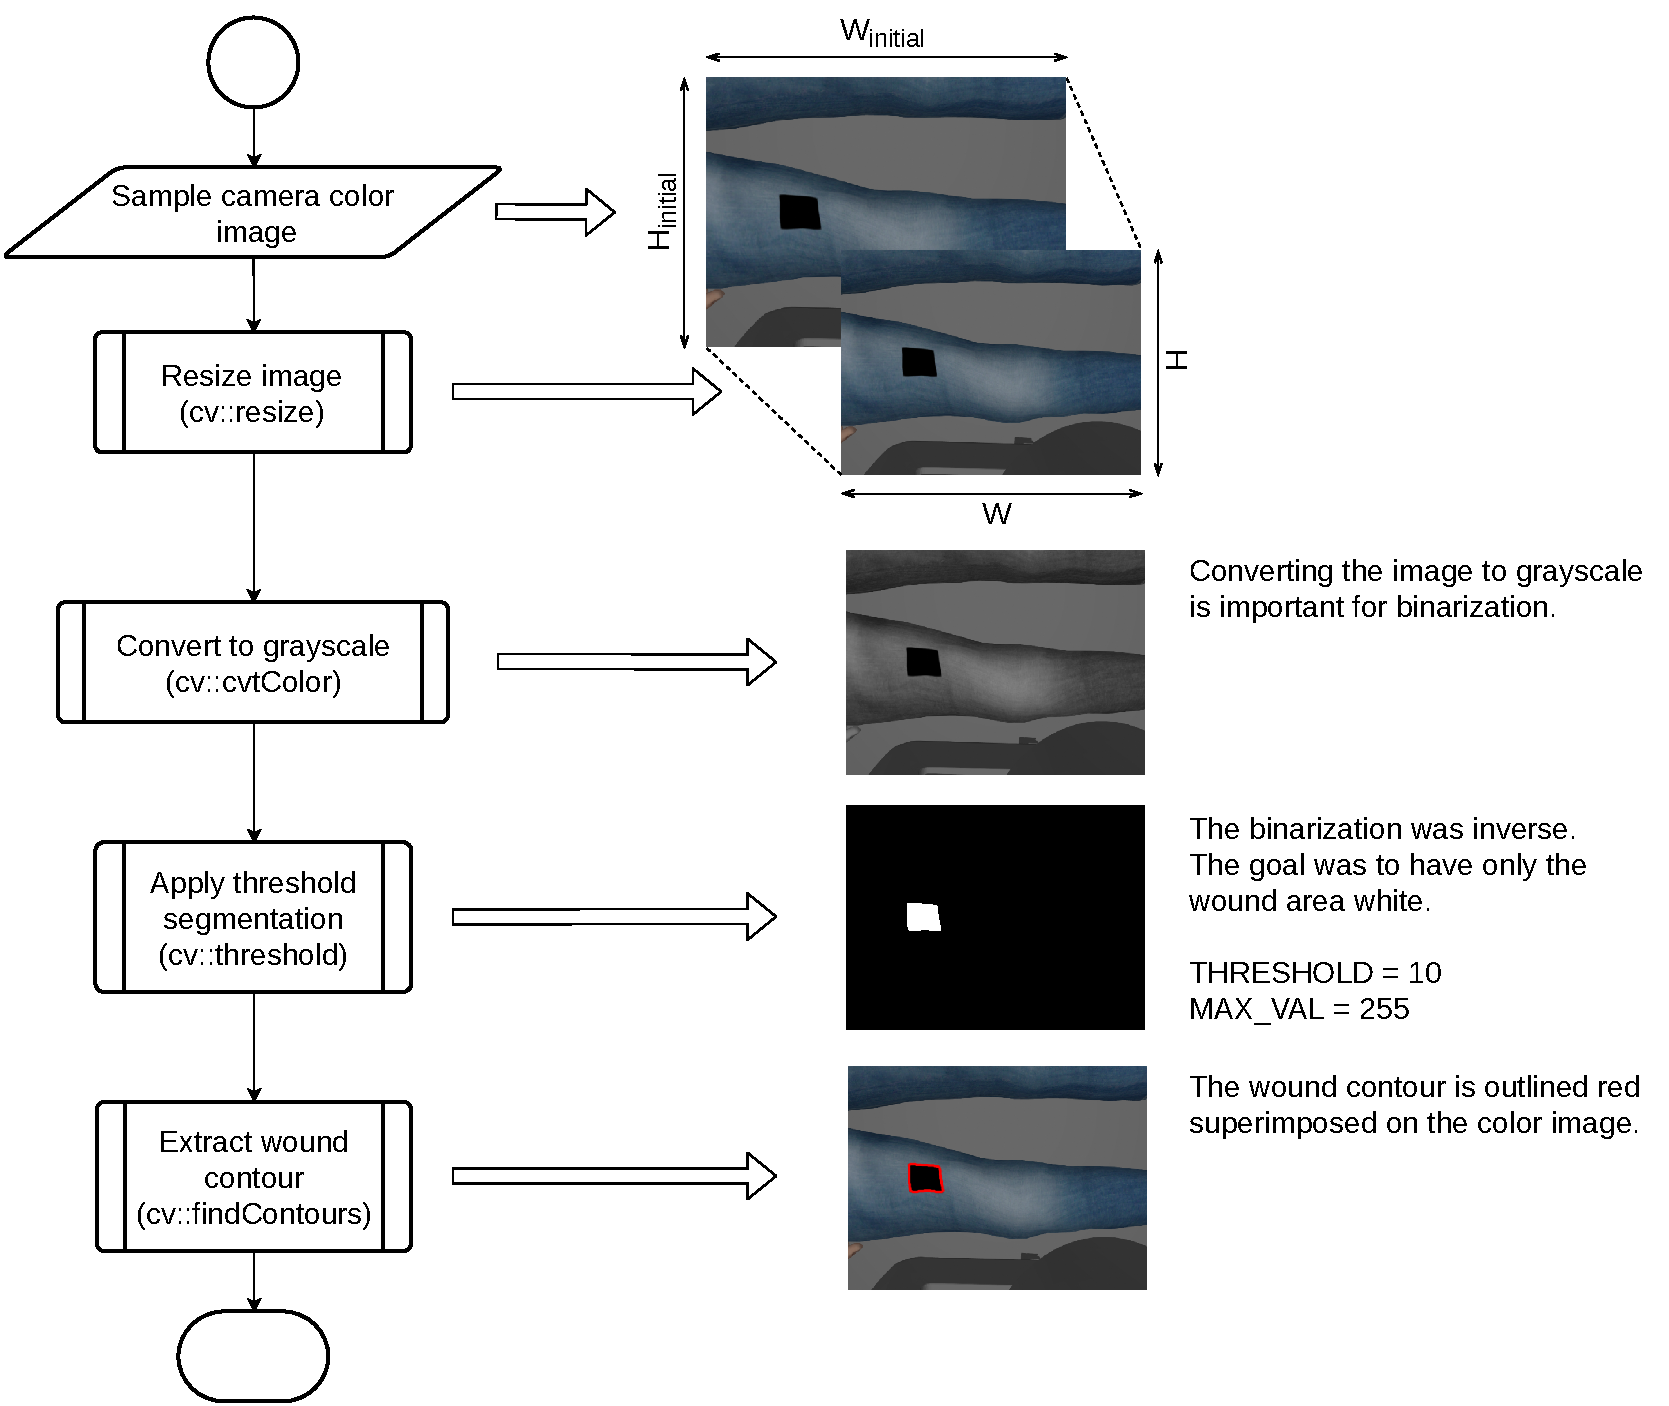
\includegraphics[width=\textwidth]{system_architecture_layer_wound_detection_segmentation_flowchart}
	\caption{dwfdfsfsdf}
	\label{fig:system_architecture_layer_wound_detection_segmentation_flowchart}
\end{figure}

The wound detection is done over the camera RGB data stream. Since we intend to use a binarization approach, first we need to change the color space from RGB to grayscale. This conversion corresponds to a weighted sum of the three color channels, pixel by pixel (see eq. \ref{eq:convertion_rgb_grayscale_general}).

\begin{equation}
\boldsymbol{I}_{GRAY}(x,y) = r * \boldsymbol{R}(x,y) + g * \boldsymbol{G}(x,y) + b * \boldsymbol{B}(x,y)
\label{eq:convertion_rgb_grayscale_general}
\end{equation}

where $r$, $g$ and $b$ are the weights of red, green and blue channels, respectively. The algorithm applied uses the following coefficients {\color{red} referência a estes valores...}: 
$$ r = 0.299, g = 0.587, b = 0.144 $$

After obtaining the grayscale image, a binarization algorithm is applied to convert the image to black and white. The algorithm consists on using an threshold value chosen empirically and change each pixel value according to it. If the pixel value is greater than the threshold it is converted to 0, otherwise to 1.  

Because the wound model is a black mark on a lighter background, it is easier to detect the wound contour. {\color{red} Falar sobre o algoritmo.}\\

One of the advantages of this layered structure is that it allows us to change the implementation of a specific layer and leave the rest of the stack intact. In this particular case, a simplistic algorithm is used to test the whole chain, but once it is working, another more robust algorithm can be used instead.

% subsubsection system_architectural_camera_layers_wound_detection_segmentation

\subsubsection*{Spatial Data Processing}
\label{subsubsec:system_architectural_camera_layers_spatial_data}

After the wound is detected by the previous layer, this layer is responsible for obtaining spatial data from the wound contour. At this level the wound position, contour area and perimeter and contour mesh are obtained. Figure \ref{fig:system_architecture_layer_camera_spatial_data_flowchart} presents the flowchart of spatial data processing.

\begin{figure}[htbp]
	\centering
	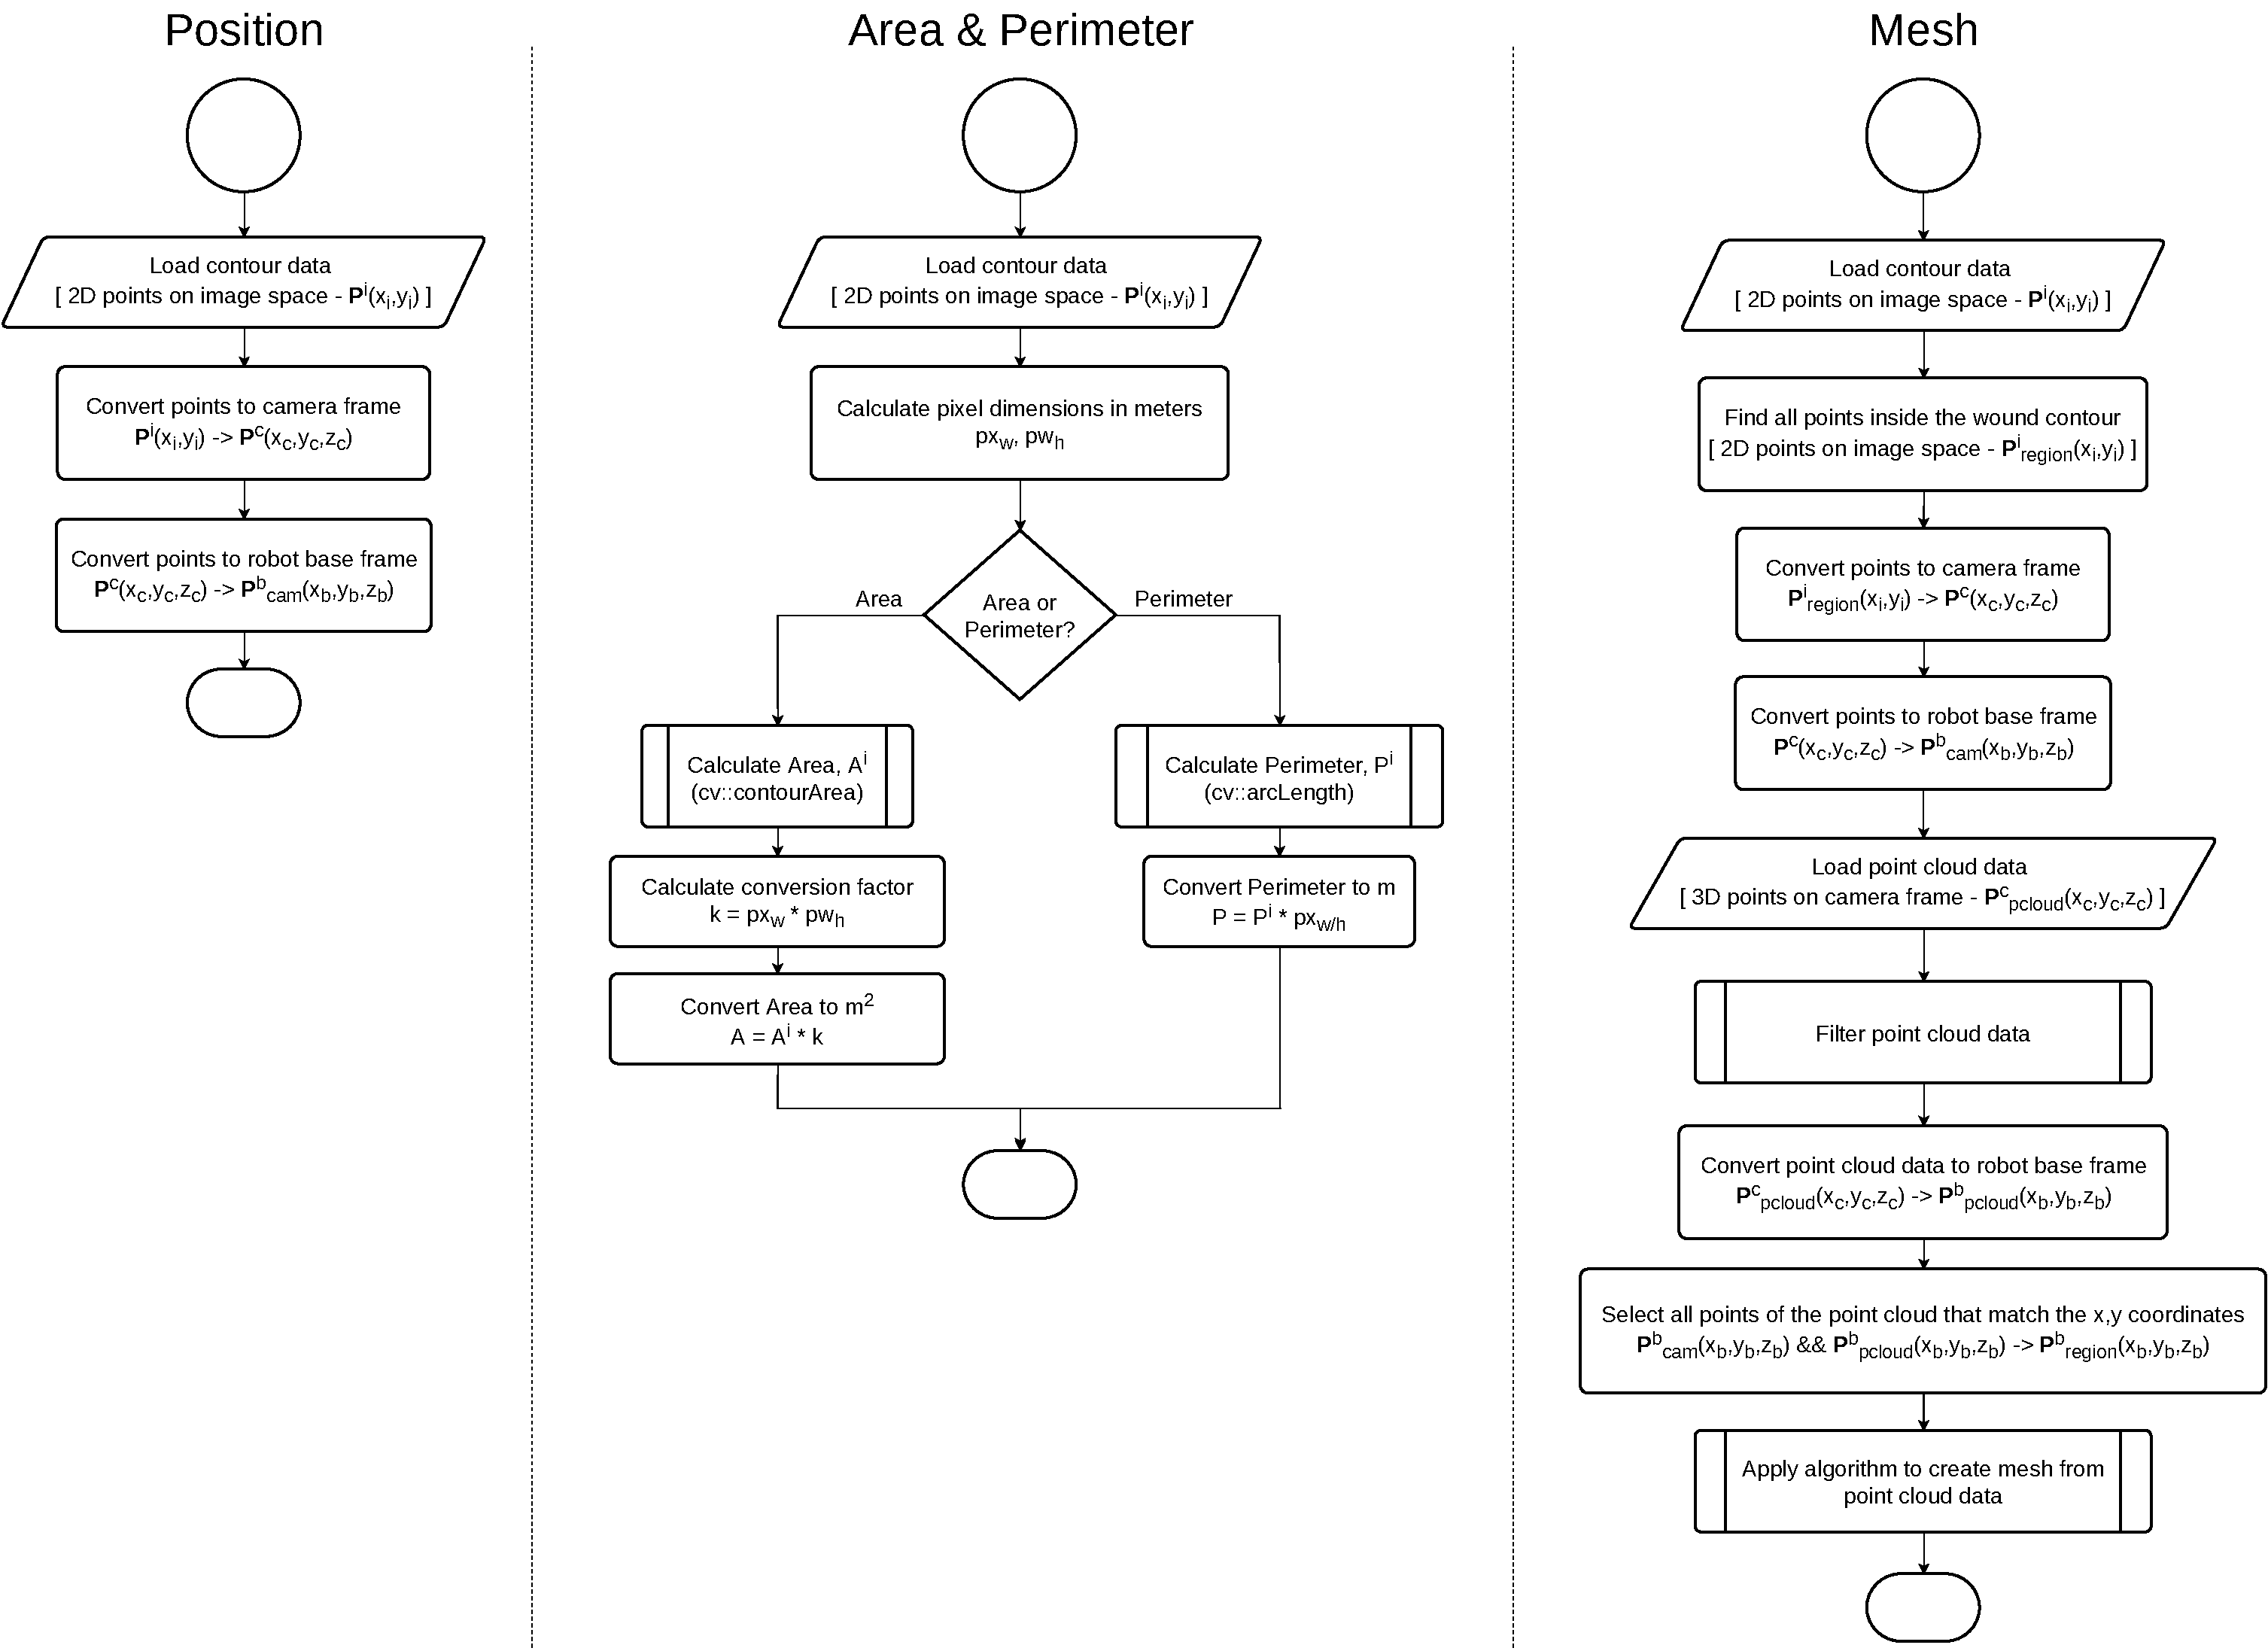
\includegraphics[width=\textwidth]{system_architecture_layer_camera_spatial_data_flowchart}
	\caption{sdfsdfsdfsd}
	\label{fig:system_architecture_layer_camera_spatial_data_flowchart}
\end{figure}

The position of the wound is given by the contour previously obtained. The contour is a set of 2D points on the image space. To obtain the position of each point in relation to the robot, a transform must be applied between the camera reference frame ($O_cx_cy_cz_c$) and the robot base frame ($O_bx_by_bz_b$).

A point $\boldsymbol{P}^c = (x_c, y_c, z_c)$, on the camera frame, is transformed to point $\boldsymbol{P}^b = (x_b, y_b, z_b)$, on the robot base frame, according to equation \ref{eq:camera_point_transform_robot_base_camera},

\begin{equation}
\boldsymbol{P}^b = \boldsymbol{H}^b_c \boldsymbol{P}^c
\label{eq:camera_point_transform_robot_base_camera}
\end{equation}

where $\boldsymbol{H}^b_c$ is the homogeneous transformation matrix between camera frame and robot base frame. Knowing every point of the wound contour allows us to precisely know the wound location.\\

The wound area and perimeter are calculated on the image space (px$^2$, px) and converted to robot space (\si{\meter \squared}, \si{\meter}). The conversion factor, $k$, is obtained by relating the image dimensions with the \gls{hfov} at a certain camera distance. $k$ allows to convert the area dimensions. For the perimeter, only $px_w$ or $px_h$ is needed. Equations \ref{eq:px_to_meter_conversion} and \ref{eq:workspace_limits} show the conversion factor calculation.

\begin{equation}
k = px_w \times px_h = (\frac{Y_{max} - Y_{min}}{W}) \times (\frac{X_{max} - X_{min}}{H})
\label{eq:px_to_meter_conversion}
\end{equation}

\begin{equation}
\label{eq:workspace_limits}
    \left.
    \begin{aligned}
        Y_{max} = \frac{W_s}{2} \\
        Y_{min} = \frac{-W_s}{2} \\
        X_{max} = \frac{H_s}{2} \\
        X_{min} = \frac{-H_s}{2} \\
    \end{aligned}
    \right.
\end{equation}

The quantities $W_s$ and $H_s$ represent the width and height, respectively, of the projected image at a certain distance from the camera (Fig. \ref{fig:}).

\begin{figure}[htbp]
	\centering
	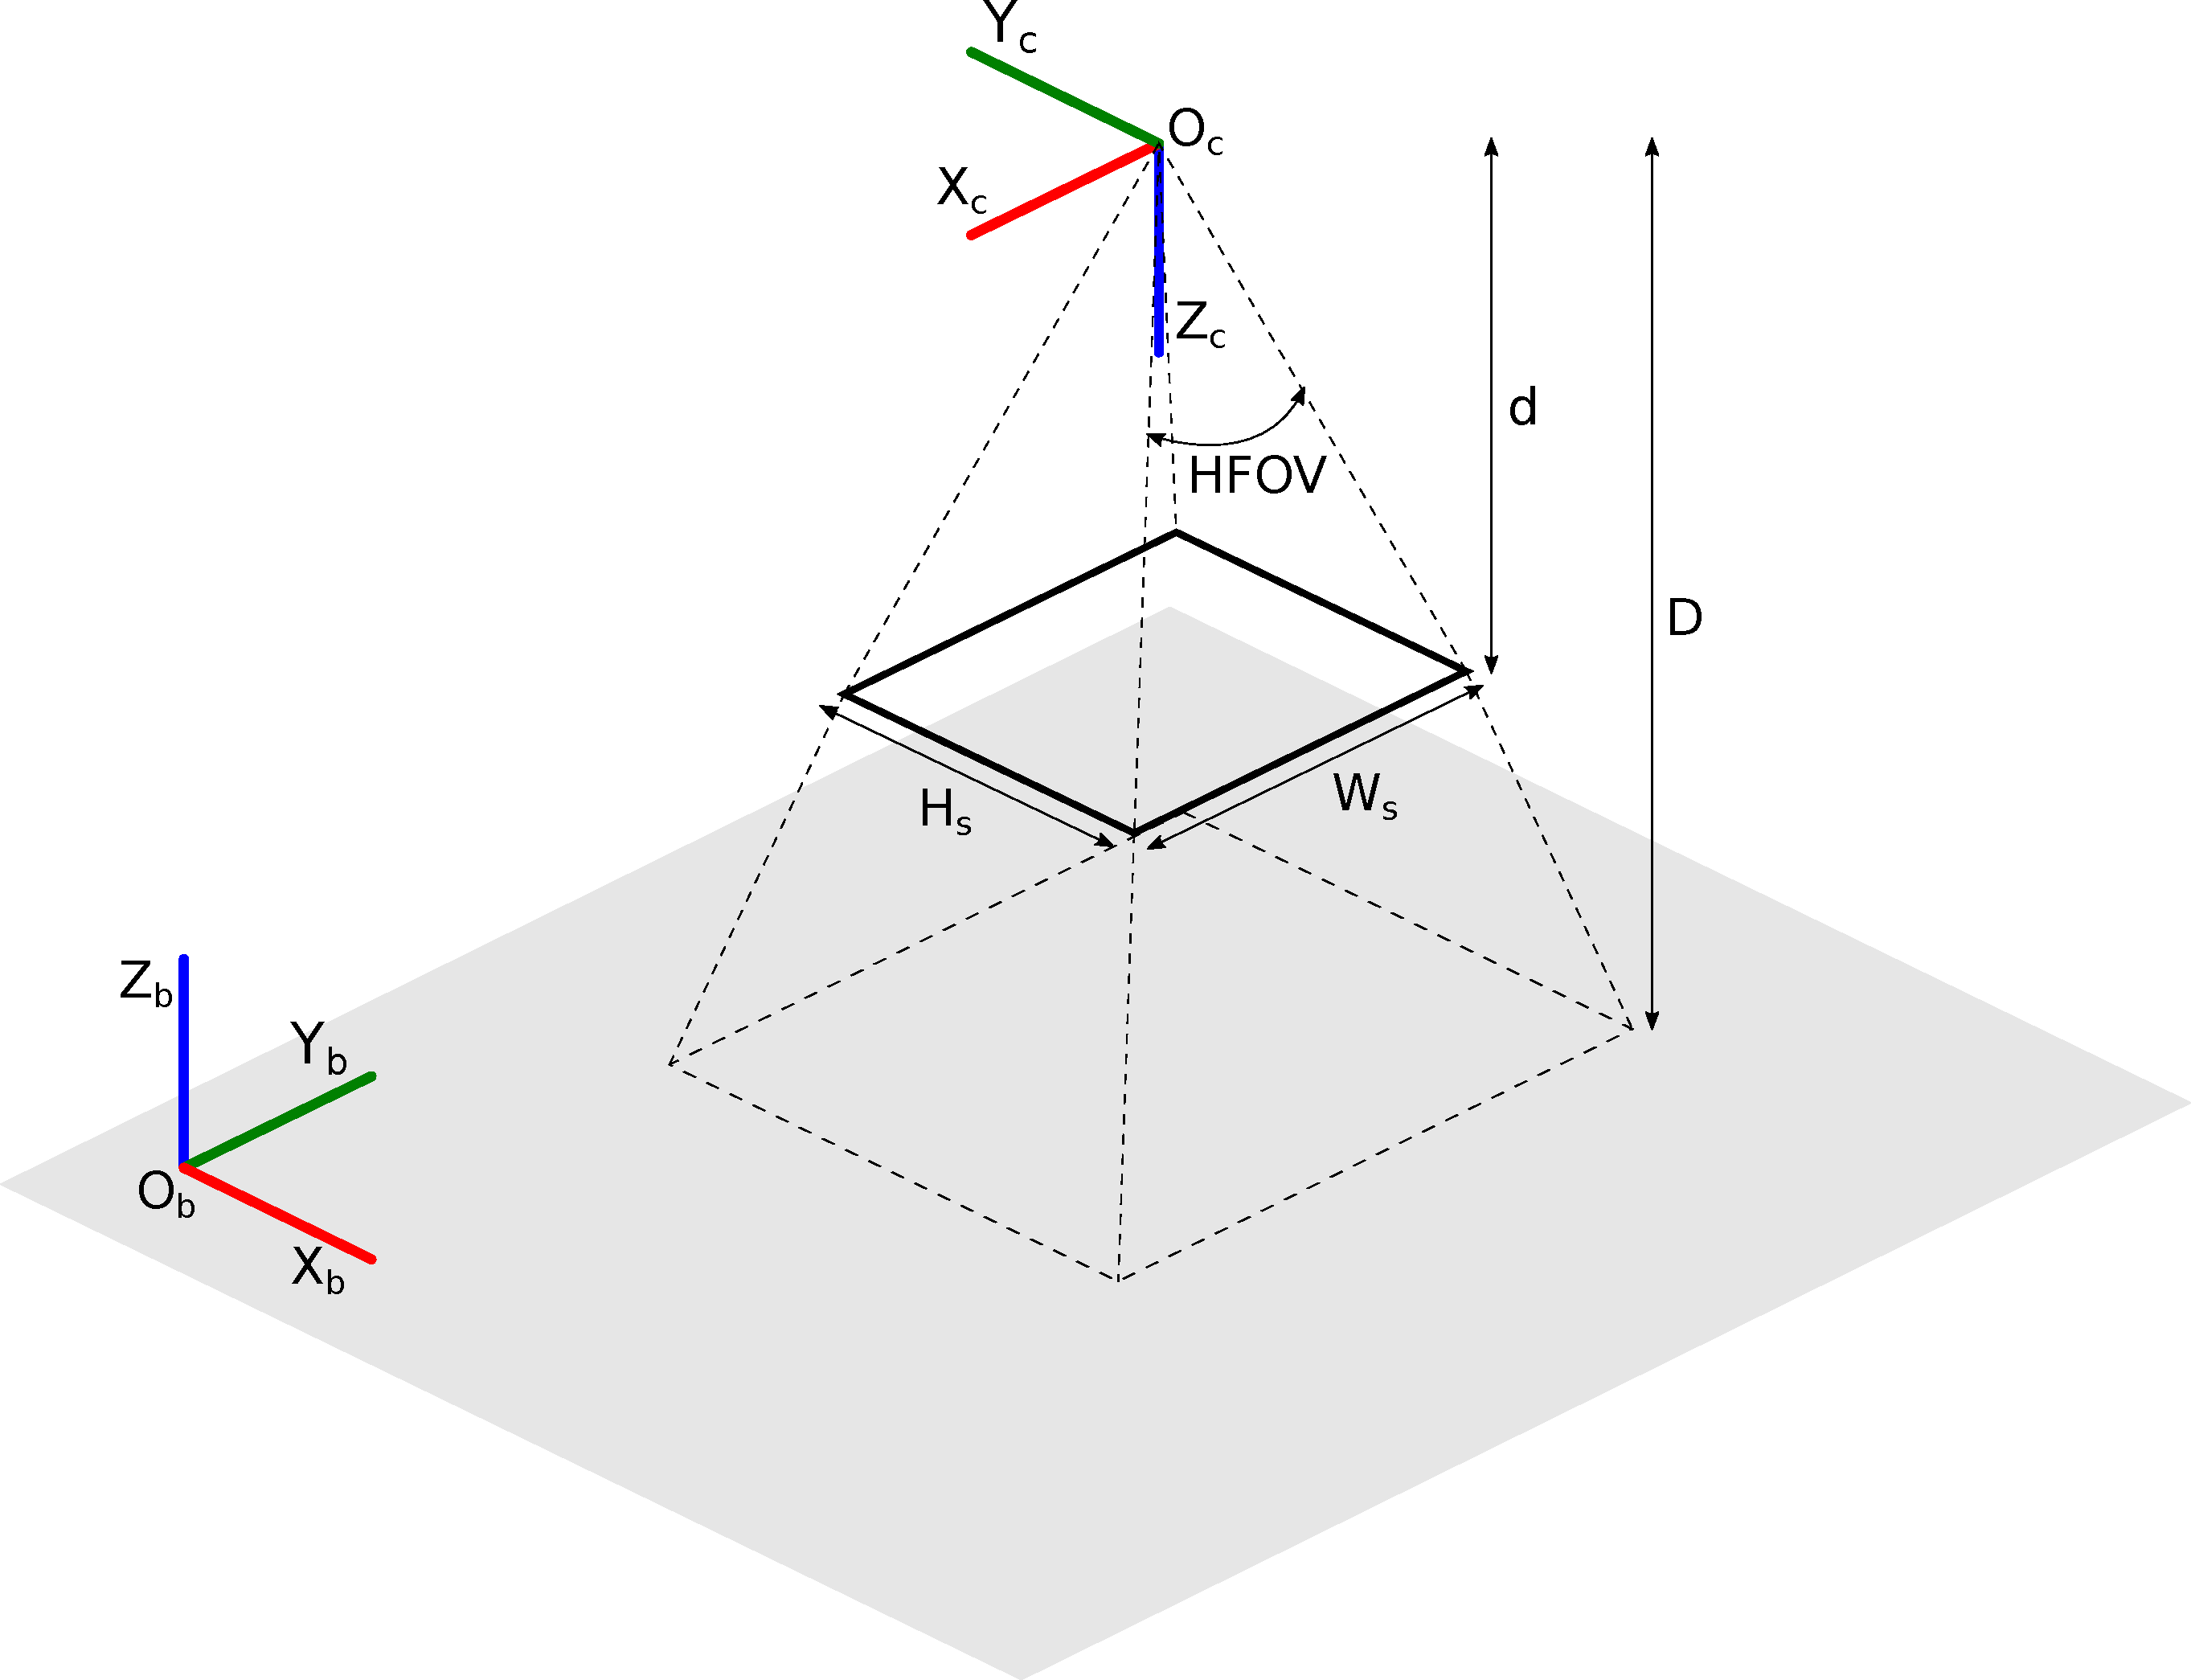
\includegraphics[width=\textwidth]{system_architecture_layer_camera_spatial_data_image_wsp_dimensions}
	\caption{sfsdfsdfsdfsd}
	\label{fig:system_architecture_layer_camera_spatial_data_image_wsp_dimensions}
\end{figure}

According to the camera specifications, at a certain resolution there is an associated \gls{hfov} in radians. By multiplying this \gls{hfov} with a distance $d$, from the camera to an object, we get the image width in meters ($W_s$). Having the width and knowing the resolution, we can easily obtain the height ($H_s$). In resume (\ref{eq:image_dimension_in_meters}),

\begin{equation}
\label{eq:image_dimension_in_meters}
    \left.
    \begin{aligned}
        r = \frac{W}{H} \\
        W_s = HFOV \times d \\
        H_s = \frac{W_s}{r} \\
    \end{aligned}
    \right.
\end{equation}

Lastly, this layer also obtains a mesh of the detected wound for possible geometrical analysis.

The mesh is obtained by intersecting the point cloud data with the image segmentation data. The point cloud data is reduced by using a box filter and point density reduction. The box filter uses $W_s$, $H_s$ and $d$ to limit x, y and z. The point density is reduced to a minimum distance between points of 5 \si{\milli \meter} in all axes (Fig. \ref{fig:system_architecture_layer_camera_spatial_data_mesh_generation}). All the pixels inside the wound contour are selected and converted to the robot base frame (see \ref{eq:camera_point_transform_robot_base_camera}). Afterwards, these points are used to filter the point cloud 3D points to select only the desired region (Fig. \ref{fig:system_architecture_layer_camera_spatial_data_mesh_generation}).

After the point cloud data is filtered, an algorithm is applied to calculate the surface normals and mesh triangulation. The final result is stored in file, using the \textbf{Polygon File Format} or \textbf{Stanford Triangle Format}. This file format uses the extension \textbf{ply}.

\begin{figure}[htbp]
	\centering
	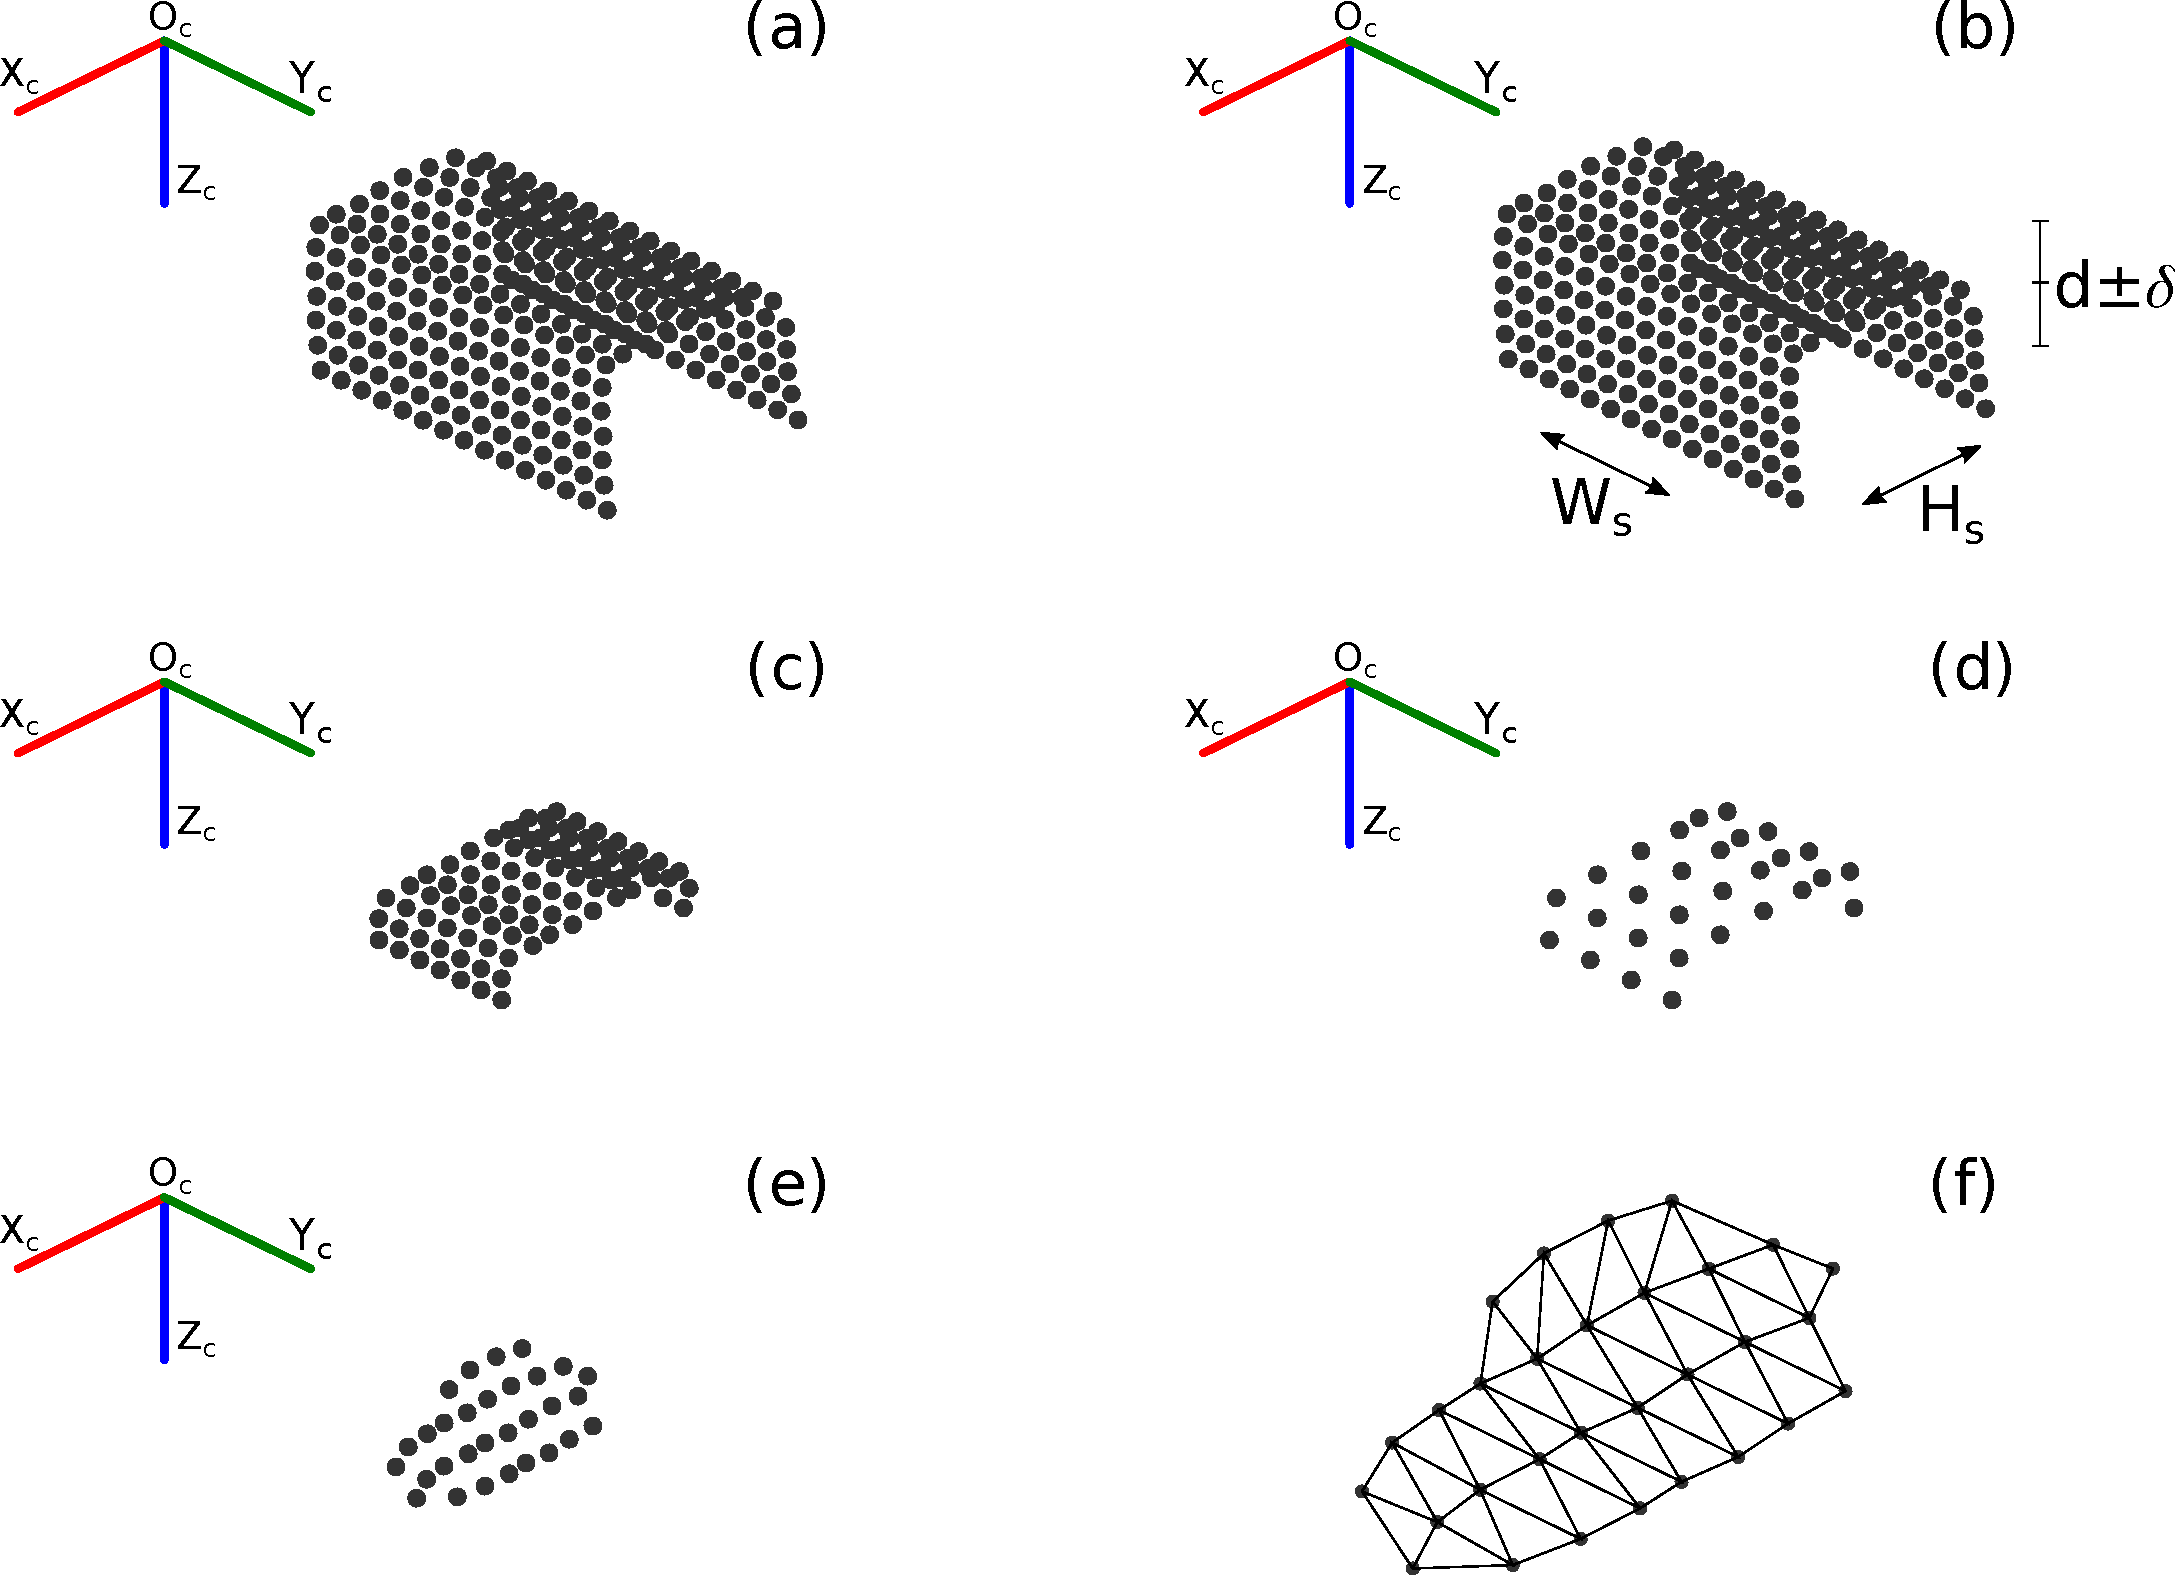
\includegraphics[width=\textwidth]{system_architecture_layer_camera_spatial_data_mesh_generation}
	\caption{sfsdfsdfsdfsd}
	\label{fig:system_architecture_layer_camera_spatial_data_mesh_generation}
\end{figure}

% subsubsection system_architectural_camera_layers_spatial_data

% subsection system_architectural_camera_layers

\subsection{Robot Layers}
\label{subsec:system_architectural_robot_layers}

\subsubsection*{Spatial Data Processing}
\label{subsubsec:system_architectural_robot_layers_spatial_data}

% subsubsection system_architectural_robot_layers_spatial_data

\subsubsection*{Path Planning}
\label{subsubsec:system_architectural_robot_layers_path_planning}

% subsubsection system_architectural_robot_layers_path_planning

\subsubsection*{Trajectory Definition}
\label{subsubsec:system_architectural_robot_layers_trajectory_definition}

% subsubsection system_architectural_robot_layers_trajectory_definition

\subsubsection*{Visual Servoing \& Control}
\label{subsubsec:system_architectural_robot_layers_visual_servoing_control}

% subsubsection system_architectural_robot_layers_visual_servoing_control

% subsection system_architectural_robot_layers

\subsection{Print Head Layers}
\label{subsec:system_architectural_printhead_layers}

\subsubsection*{Bioink Management}
\label{subsubsec:system_architectural_printhead_layers_bioink_management}

% subsubsection system_architectural_printhead_layers_bioink_management

\subsubsection*{Bioink Dispensing Control}
\label{subsubsec:system_architectural_printhead_layers_bioink_dispensing_control}

% subsubsection system_architectural_printhead_layers_bioink_dispensing_control

% subsection system_architectural_printhead_layers